% ============================================================
%  TextBlob-Based Polarity Pseudo-Labelling for CMU-MOSI
%  A Complete Research Paper with Algorithms, Proofs & Flowcharts
% ============================================================
\documentclass[12pt,a4paper]{article}

% ── Core packages ───────────────────────────────────────────
\usepackage[T1]{fontenc}
\usepackage[utf8]{inputenc}
% lmodern not available; using default CM fonts
\usepackage[margin=2.5cm]{geometry}
\usepackage[activate=false,tracking=false]{microtype}
\usepackage{setspace}
\onehalfspacing

% ── Math ────────────────────────────────────────────────────
\usepackage{amsmath,amssymb,amsthm,mathtools}
\usepackage{bm}

% ── Theorem environments ────────────────────────────────────
\theoremstyle{plain}
\newtheorem{theorem}{Theorem}[section]
\newtheorem{lemma}[theorem]{Lemma}
\newtheorem{proposition}[theorem]{Proposition}
\newtheorem{corollary}[theorem]{Corollary}

\theoremstyle{definition}
\newtheorem{definition}[theorem]{Definition}
\newtheorem{axiom}[theorem]{Axiom}
\newtheorem{example}[theorem]{Example}
\newtheorem{remark}[theorem]{Remark}

% ── Algorithms ──────────────────────────────────────────────
\usepackage{algorithm}
\usepackage{algpseudocode}
\algrenewcommand\algorithmicrequire{\textbf{Input:}}
\algrenewcommand\algorithmicensure{\textbf{Output:}}
\algnewcommand{\LineComment}[1]{\State \(\triangleright\) #1}

% ── TikZ / PGF ──────────────────────────────────────────────
\usepackage{tikz}
\usetikzlibrary{
  shapes.geometric, shapes.misc, shapes.arrows,
  arrows.meta, positioning, fit, calc,
  shadows, backgrounds, patterns,
  decorations.pathreplacing, decorations.markings,
  matrix, chains, scopes, fadings
}

% ── Tables, listings, graphics ──────────────────────────────
\usepackage{booktabs,multirow,tabularx,array}
\usepackage{xcolor}
\usepackage{graphicx}
\usepackage{subcaption}
\usepackage{listings}
\usepackage{enumitem}
\usepackage{hyperref}
\hypersetup{colorlinks=true, linkcolor=NavyBlue,
            citecolor=ForestGreen, urlcolor=Maroon}
\usepackage[capitalise,nameinlink]{cleveref}

% ── Bibliography ────────────────────────────────────────────
\usepackage[numbers,sort&compress]{natbib}

% ── Custom colours ──────────────────────────────────────────
\definecolor{NavyBlue}{HTML}{003366}
\definecolor{ForestGreen}{HTML}{228B22}
\definecolor{Maroon}{HTML}{800000}
\definecolor{LightBlue}{HTML}{DDEEFF}
\definecolor{LightGreen}{HTML}{DDFFDD}
\definecolor{LightRed}{HTML}{FFDDDD}
\definecolor{LightYellow}{HTML}{FFFACC}
\definecolor{LightGrey}{HTML}{F5F5F5}
\definecolor{DarkGrey}{HTML}{444444}
\definecolor{AccentOrange}{HTML}{FF6600}
\definecolor{AccentPurple}{HTML}{6600CC}

% ── TikZ styles ─────────────────────────────────────────────
\tikzset{
  % Decision diamond
  decision/.style={
    diamond, draw=NavyBlue, thick,
    fill=LightBlue, text width=4em,
    text badly centered, inner sep=0pt,
    aspect=2, drop shadow
  },
  % Process rectangle
  process/.style={
    rectangle, draw=ForestGreen, thick,
    fill=LightGreen, text width=9em,
    text centered, minimum height=3em,
    rounded corners=2pt, drop shadow
  },
  % Start/End oval
  startstop/.style={
    ellipse, draw=Maroon, thick,
    fill=LightRed, text width=7em,
    text centered, minimum height=2.5em,
    drop shadow
  },
  % Data parallelogram
  io/.style={
    trapezium, trapezium left angle=70,
    trapezium right angle=110,
    draw=AccentOrange, thick,
    fill=LightYellow, text width=8em,
    text centered, minimum height=2.5em,
    drop shadow
  },
  % Annotation box
  annot/.style={
    rectangle, draw=DarkGrey, dashed,
    fill=LightGrey, text width=11em,
    text centered, minimum height=2em,
    font=\footnotesize\ttfamily,
    rounded corners=1pt
  },
  % Arrow style
  arrow/.style={
    -Stealth, thick, draw=DarkGrey
  },
  % Example node
  example_node/.style={
    rectangle, draw=AccentPurple, thick,
    fill=white, text width=12em,
    text centered, minimum height=2.5em,
    rounded corners=3pt,
    font=\footnotesize
  },
  % Output node
  output_node/.style={
    rectangle, draw=Maroon, thick,
    fill=LightRed!50, text width=12em,
    text centered, minimum height=2.5em,
    rounded corners=3pt,
    font=\footnotesize\bfseries
  }
}

% ── Listing style ────────────────────────────────────────────
\lstset{
  language=Python,
  basicstyle=\footnotesize\ttfamily,
  keywordstyle=\color{NavyBlue}\bfseries,
  commentstyle=\color{ForestGreen}\itshape,
  stringstyle=\color{Maroon},
  showstringspaces=false,
  breaklines=true,
  frame=single,
  framesep=4pt,
  backgroundcolor=\color{LightGrey},
  numbers=left,
  numberstyle=\tiny\color{DarkGrey},
  numbersep=8pt,
  tabsize=4,
  captionpos=b
}

% ── Title metadata ───────────────────────────────────────────
\title{%
  \textbf{Rule-Based Polarity Pseudo-Labelling for\\
  Multimodal Sentiment Analysis:\\[4pt]
  A Formal Treatment of the TextBlob Algorithm\\
  Applied to CMU-MOSI}\\[8pt]
  {\large Technical Research Paper — MIVA-KNIGHT Pipeline E}
}

\author{%
  Oluwakayode Soyinka\\
  \small IT 581 Capstone Project, Concordia University of Edmonton\\
  \small Supervised by Dr.\ Baidya Saha
}

\date{\today}

% ============================================================
\begin{document}
% ============================================================

\maketitle
\thispagestyle{empty}

\begin{abstract}
  This paper provides a rigorous and exhaustive formal treatment of the
  \emph{TextBlob polarity pseudo-labelling} algorithm used in Cell~4 of
  the MIVA-KNIGHT Pipeline~E notebook for multimodal sentiment fusion on
  CMU-MOSI.  Because the canonical CMU-MOSI gold labels are gated behind
  a proprietary \texttt{.pkl} file, Pipeline~E derives sentiment targets
  from raw transcript text using TextBlob's rule-based lexicon–pattern
  system.  We formalise the entire computational pathway: from raw Unicode
  string ingestion, through morphological normalisation and Part-of-Speech
  (POS) tagging, through lexicon lookup and pattern-modifier application,
  to the final clipped linear scaling that maps the TextBlob
  $[-1,+1]$ range onto the CMU-MOSI $[-3,+3]$ annotation scale.  We
  provide axiomatic foundations, lemmas and theorems governing convergence
  and label quality, formal pseudocode algorithms, and a fully annotated
  TikZ inference flowchart in which every node carries a concrete
  running example derived from a real CMU-MOSI transcript utterance.
  The paper closes with an empirical analysis of the label distribution,
  a comparison with alternative pseudo-labelling strategies, and a
  discussion of downstream effects on the Multimodal Fusion Transformer
  trained on these labels.
\end{abstract}

\tableofcontents
\newpage

% ============================================================
\section{Introduction}
\label{sec:intro}
% ============================================================

Multimodal sentiment analysis is the task of predicting the emotional
valence of a human utterance from its textual, acoustic, and visual
modalities simultaneously.  The CMU-MOSI corpus~\citep{zadeh2016mosi}
provides $2{,}199$ video segments from YouTube opinion reviews, each
annotated by five crowd-sourced workers on a continuous $[-3,+3]$ scale
where $-3$ denotes \emph{strongly negative} and $+3$ denotes
\emph{strongly positive}.  The final gold label for each segment is the
\emph{mean} of the five annotations.

\subsection{Motivation: The Missing \texttt{.pkl} Problem}

The official CMU-MOSI labels are distributed as a serialised Python
pickle file (\texttt{CMU\_MOSI\_Opinion\_Labelled\_Raw.pkl}) that
requires PhysioNet credentialing.  In the MIVA-KNIGHT project
environment the pickle file was unavailable at training time.
Pipeline~E therefore adopts a \emph{pseudo-labelling} strategy: for
each segment the sentiment label is computed automatically from the
segment's transcript text using TextBlob's rule-based polarity scorer.

\subsection{Scope and Contributions}

This paper makes the following contributions:
\begin{enumerate}[label=(\arabic*)]
  \item A \textbf{formal axiomatic model} of the TextBlob polarity
        function, including its lexicon, POS pattern rules, and
        aggregation operator (\cref{sec:formal}).
  \item \textbf{Lemmas and theorems} establishing range bounds, monoton-
        icity properties, and the asymptotic quality of the
        pseudo-labels with respect to true crowd-sourced labels
        (\cref{sec:theory}).
  \item \textbf{Formal pseudocode algorithms} with full complexity
        analysis for \texttt{build\_samples()} and its constituent
        subroutines (\cref{sec:algorithms}).
  \item A \textbf{fully annotated TikZ inference flowchart} tracing a
        concrete CMU-MOSI utterance through every computational step,
        showing both intermediate values and final outputs at each node
        (\cref{sec:flowchart}).
  \item \textbf{Empirical analysis} of the resulting label distribution,
        class balance, and downstream training dynamics
        (\cref{sec:empirical}).
\end{enumerate}

% ============================================================
\section{Background}
\label{sec:background}
% ============================================================

\subsection{The CMU-MOSI Dataset}

CMU-MOSI contains $93$ YouTube videos from $89$ distinct speakers.
Each video is segmented into utterances at natural sentence boundaries,
yielding $2{,}199$ segments.  The standard three-way split is:
\begin{itemize}
  \item \textbf{Train:} $59$ video IDs, $1{,}521$ segments.
  \item \textbf{Valid:} $15$ video IDs, $314$ segments.
  \item \textbf{Test:} $19$ video IDs, $364$ segments.
\end{itemize}

Splits are \emph{video-level} (never segment-level) to prevent data
leakage: all segments from the same speaker/recording appear in
exactly one partition.

\subsection{TextBlob: Architecture Overview}

TextBlob is a Python NLP library built on top of NLTK and the
\emph{Pattern} library~\citep{de2012pattern}.  Its sentiment analysis
module implements a rule-based \emph{lexicon–pattern} system that
assigns two real-valued scores to any English sentence:

\begin{definition}[TextBlob Sentiment Tuple]
\label{def:tb_sentiment}
  For a string $s$, TextBlob returns
  $\text{TextBlob}(s).\text{sentiment} = (p, q)$
  where $p \in [-1,+1]$ is the \emph{polarity} and
  $q \in [0,+1]$ is the \emph{subjectivity}.
  This paper concerns only the polarity component $p$.
\end{definition}

\subsection{The TextBlob Lexicon}

TextBlob's core lexicon is the \emph{Pattern sentiment dictionary}
(\texttt{en-sentiment.xml}), which maps individual English word types
to numerical sentiment values.  Each entry has the form:
\[
  \mathcal{L} : w \mapsto (p_w,\, q_w,\, \text{POS}_w,\,
                            \text{sense}_w)
\]
where $w$ is the lowercase lemma, $p_w \in [-1,+1]$ the intrinsic
polarity, $q_w \in [0,+1]$ the intrinsic subjectivity, $\text{POS}_w$
the expected part-of-speech tag, and $\text{sense}_w$ an optional
WordNet sense identifier.

\begin{example}[Lexicon Entries]
\label{ex:lexicon}
  Selected entries from the Pattern lexicon relevant to CMU-MOSI:
  \begin{center}
    \begin{tabular}{llll}
      \toprule
      Lemma & Polarity & Subjectivity & POS \\
      \midrule
      \textit{love}      & $+0.500$ & $0.600$ & verb \\
      \textit{great}     & $+0.800$ & $0.750$ & adjective \\
      \textit{terrible}  & $-0.625$ & $1.000$ & adjective \\
      \textit{not}       & ---      & ---     & (negator) \\
      \textit{very}      & ---      & ---     & (intensifier) \\
      \textit{boring}    & $-0.250$ & $0.625$ & adjective \\
      \textit{excited}   & $+0.400$ & $0.600$ & adjective \\
      \bottomrule
    \end{tabular}
  \end{center}
\end{example}

% ============================================================
\section{Formal Model}
\label{sec:formal}
% ============================================================

We now build the formal algebraic model of TextBlob's polarity
computation step by step.

\subsection{String Normalisation}

\begin{axiom}[Case Folding]
\label{ax:casefolding}
  The polarity function is defined over lowercase strings.  For any
  string $s$, Pipeline~E applies
  $\hat{s} = \textsc{LowerCase}(s)$
  before invoking TextBlob, i.e.\ $\text{polarity}(s) =
  \text{polarity}(\hat{s})$.
\end{axiom}

\begin{axiom}[Tokenisation Determinism]
\label{ax:tokendet}
  TextBlob's tokeniser is deterministic: for any fixed string $s$,
  repeated calls produce the identical token sequence
  $\mathbf{w} = (w_1, w_2, \ldots, w_n)$.
\end{axiom}

\begin{definition}[Tokenisation Function]
\label{def:tokenise}
  Let $\Sigma^*$ denote the set of Unicode strings.  The TextBlob
  tokeniser is a function
  \[
    \tau : \Sigma^* \to \mathcal{W}^*
  \]
  where $\mathcal{W}$ is the vocabulary of English word types.  In
  practice $\tau$ applies:
  \begin{enumerate}[label=(\roman*)]
    \item Unicode normalisation (NFC form),
    \item contraction expansion (e.g.\ \textit{don't}
          $\to$ \textit{do}, \textit{n't}),
    \item punctuation stripping,
    \item whitespace splitting.
  \end{enumerate}
\end{definition}

\subsection{POS Tagging}

\begin{definition}[POS Tag Function]
\label{def:pos}
  Given a token sequence $\mathbf{w} = (w_1,\ldots,w_n)$, TextBlob
  applies the averaged-perceptron POS tagger (trained on Penn Treebank)
  to produce a tagged sequence
  \[
    \rho(\mathbf{w}) =
    \bigl((w_1, t_1), (w_2, t_2), \ldots, (w_n, t_n)\bigr)
  \]
  where each $t_i \in \mathcal{T}$ is a Penn Treebank POS tag
  (e.g.\ \texttt{JJ}, \texttt{RB}, \texttt{NN}, \texttt{VB}).
\end{definition}

\begin{definition}[Coarse POS Projection]
\label{def:coarsepos}
  TextBlob maps Penn tags to Pattern-library coarse POS tags via the
  surjective function $\phi : \mathcal{T} \to \{$\texttt{JJ, RB, NN,
  VB, CC, IN}$\}$:
  \[
    \phi(t) =
    \begin{cases}
      \texttt{JJ} & t \in \{\texttt{JJ}, \texttt{JJR}, \texttt{JJS}\} \\
      \texttt{RB} & t \in \{\texttt{RB}, \texttt{RBR}, \texttt{RBS}\} \\
      \texttt{NN} & t \in \{\texttt{NN}, \texttt{NNS}, \texttt{NNP},
                             \texttt{NNPS}\} \\
      \texttt{VB} & t \in \{\texttt{VB}, \texttt{VBD}, \texttt{VBG},
                             \texttt{VBN}, \texttt{VBP}, \texttt{VBZ}\} \\
      \texttt{CC} & t = \texttt{CC} \\
      \texttt{IN} & \text{otherwise}
    \end{cases}
  \]
\end{definition}

\subsection{Lexicon Lookup}

\begin{definition}[Lemmatisation]
\label{def:lemma}
  TextBlob's NLTK-based lemmatiser $\ell : \mathcal{W} \times
  \mathcal{T} \to \mathcal{W}$ maps each surface word form to its
  base lemma, conditioned on POS:
  \[
    \ell(w, t) =
    \text{WordNetLemmatizer.lemmatize}(w,\, \phi(t))
  \]
  For example, $\ell(\textit{movies}, \texttt{NN}) = \textit{movie}$
  and $\ell(\textit{loved}, \texttt{VB}) = \textit{love}$.
\end{definition}

\begin{definition}[Lexicon Score Function]
\label{def:lexlookup}
  The base polarity score for a word $w$ with POS $t$ is:
  \[
    \sigma(w, t) =
    \begin{cases}
      p_{\ell(w,t)} & \text{if } \ell(w,t) \in \mathcal{L}
                       \text{ and POS matches} \\
      0             & \text{otherwise}
    \end{cases}
  \]
  where $p_{\cdot}$ is the polarity value stored in the Pattern lexicon
  $\mathcal{L}$.
\end{definition}

\subsection{Modifier Rules}

TextBlob inherits Pattern's \emph{modifier pattern system}, which
identifies adverbs and negators in the context window of each scored
word and adjusts the base score accordingly.

\begin{definition}[Context Window]
\label{def:window}
  For word position $i$ in sentence $\mathbf{w}$, the \emph{left
  context window} of radius $k$ is
  $\mathcal{C}_k(i) = \{w_{i-k}, w_{i-k+1}, \ldots, w_{i-1}\}$.
  TextBlob uses $k=3$.
\end{definition}

\begin{definition}[Negation Indicator]
\label{def:negation}
  The negation indicator for position $i$ is
  \[
    \delta_{\text{neg}}(i) =
    \mathbf{1}\bigl[\exists j \in \mathcal{C}_3(i):\;
      w_j \in \mathcal{N}\bigr]
  \]
  where $\mathcal{N} = \{$\textit{not, no, never, neither, nor,
  without, hardly, barely, scarcely, nothing}$\}$.
\end{definition}

\begin{definition}[Intensifier Multiplier]
\label{def:intensifier}
  The intensifier multiplier for position $i$ is
  \[
    \mu(i) =
    \begin{cases}
      1.5  & \exists j \in \mathcal{C}_3(i): w_j \in \mathcal{I}_+ \\
      0.5  & \exists j \in \mathcal{C}_3(i): w_j \in \mathcal{I}_- \\
      1.0  & \text{otherwise}
    \end{cases}
  \]
  where $\mathcal{I}_+ = \{$\textit{very, extremely, incredibly,
  really, absolutely}$\}$ and $\mathcal{I}_- = \{$\textit{somewhat,
  rather, fairly, kind of, sort of}$\}$.
\end{definition}

\begin{definition}[Adjusted Word Score]
\label{def:adjusted}
  Combining base score, negation, and intensifier:
  \[
    \tilde{\sigma}(w_i, t_i) =
    \mu(i) \cdot
    \begin{cases}
      -\sigma(w_i, t_i) & \delta_{\text{neg}}(i) = 1 \\
       \sigma(w_i, t_i) & \delta_{\text{neg}}(i) = 0
    \end{cases}
  \]
\end{definition}

\subsection{Sentence Polarity Aggregation}

\begin{definition}[Sentence Polarity]
\label{def:sentpol}
  Let $\mathcal{S} \subseteq \{1,\ldots,n\}$ be the index set of
  scored (non-zero) words.  TextBlob computes sentence polarity as
  the arithmetic mean of adjusted scores over scored words:
  \[
    P(s) =
    \begin{cases}
      \displaystyle
      \frac{1}{|\mathcal{S}|}
        \sum_{i \in \mathcal{S}} \tilde{\sigma}(w_i, t_i)
        & |\mathcal{S}| > 0 \\[8pt]
      0 & |\mathcal{S}| = 0
    \end{cases}
  \]
\end{definition}

\begin{remark}
  TextBlob processes sentences individually and then averages their
  polarity scores if the input contains multiple sentences.  For
  CMU-MOSI segments (typically one to three short sentences), this
  multi-sentence aggregation simplifies to the per-sentence formula
  above in the overwhelming majority of cases.
\end{remark}

\subsection{Linear Scaling and Clipping}

Pipeline~E maps TextBlob's $[-1,+1]$ polarity to the CMU-MOSI
$[-3,+3]$ annotation scale.

\begin{definition}[Pseudo-Label Function]
\label{def:pseudolabel}
  For a transcript string $s$, the pseudo-label $y \in [-3,+3]$ is:
  \[
    \boxed{y(s) = \text{clip}\!\left(P(s) \times 3,\; -3,\; +3\right)}
  \]
  where $\text{clip}(x, a, b) = \max(a, \min(b, x))$ and $P(s)$ is
  the TextBlob sentence polarity from \cref{def:sentpol}.
\end{definition}

\begin{definition}[Binary Label]
\label{def:binary}
  The binary sentiment label derived from $y(s)$ is:
  \[
    b(s) = \mathbf{1}[y(s) > 0]
  \]
\end{definition}

% ============================================================
\section{Theoretical Properties}
\label{sec:theory}
% ============================================================

\subsection{Range and Boundedness}

\begin{lemma}[Boundedness of Adjusted Word Score]
\label{lem:wordscore_bound}
  For any word $w_i$ and POS tag $t_i$,
  $\tilde{\sigma}(w_i, t_i) \in [-1.5,\; +1.5]$.
  \begin{proof}
    By \cref{def:lexlookup}, $\sigma(w_i, t_i) \in [-1, +1]$.
    By \cref{def:intensifier}, $\mu(i) \in \{0.5, 1.0, 1.5\}$.
    By \cref{def:adjusted}, $|\tilde{\sigma}| = \mu(i)\cdot|\sigma|
    \le 1.5 \cdot 1 = 1.5$.  The bound is attained when
    $\sigma = +1$ and $\mu = 1.5$ (or symmetrically for $-1$).
  \end{proof}
\end{lemma}

\begin{lemma}[Range of Sentence Polarity]
\label{lem:polarity_range}
  For any string $s$, $P(s) \in [-1.5,\; +1.5]$.
  \begin{proof}
    $P(s)$ is an arithmetic mean of values in $[-1.5, +1.5]$
    (by \cref{lem:wordscore_bound}).  The mean of any set of values
    drawn from a closed interval $[a,b]$ also lies in $[a,b]$.
  \end{proof}
\end{lemma}

\begin{remark}
  In practice, intensifiers rarely stack or apply to every scored
  word simultaneously, so empirical values of $P(s)$ concentrate
  in a much narrower band around $[-0.8, +0.8]$.  The theoretical
  bound of $\pm 1.5$ is a strict bound, not a typical range.
\end{remark}

\begin{theorem}[Range of Pseudo-Label]
\label{thm:label_range}
  For any transcript string $s$, $y(s) \in [-3,\; +3]$.
  \begin{proof}
    By \cref{def:pseudolabel},
    $y(s) = \text{clip}(P(s) \times 3,\; -3,\; +3)$.
    The clip function satisfies $\text{clip}(x, a, b) \in [a, b]$
    for all $x \in \mathbb{R}$, so $y(s) \in [-3, +3]$ regardless
    of the value of $P(s) \times 3$.
  \end{proof}
\end{theorem}

\begin{corollary}[Compatibility with CMU-MOSI Scale]
\label{cor:compat}
  $y(s)$ lies in the same annotation range as the official CMU-MOSI
  gold labels, making it a valid target for mean-squared-error
  regression without additional re-scaling.
\end{corollary}

\subsection{Monotonicity}

\begin{proposition}[Weak Monotonicity in Lexicon Score]
\label{prop:monotone}
  Holding all other words and context fixed, increasing the base
  lexicon polarity $p_{w_i}$ of word $w_i$ weakly increases $y(s)$.
  \begin{proof}
    $\sigma(w_i, t_i) = p_{w_i}$ (assuming the lemma matches and
    POS is compatible).  $\tilde{\sigma}(w_i,t_i)$ is a positive
    affine function of $\sigma$ when $\delta_{\text{neg}}(i) = 0$
    (and negative affine when $\delta_{\text{neg}}(i) = 1$).
    $P(s)$ is a mean that is linear in each $\tilde{\sigma}(w_i,t_i)$
    with positive weight $1/|\mathcal{S}|$.  The final clip is a
    non-decreasing function.  Composing positive-affine, positive-
    linear, and non-decreasing functions preserves the weak
    monotone relationship.
  \end{proof}
\end{proposition}

\subsection{Inversion Under Negation}

\begin{proposition}[Polarity Inversion]
\label{prop:inversion}
  If $\mathcal{N}' \subseteq \mathcal{N}$ is the set of negating
  words actually present in the three-word context of every scored
  word, then adding $\mathcal{N}'$ to an otherwise negator-free
  sentence $s$ yields a sentence $s'$ with
  $P(s') = -P(s)$.
  \begin{proof}[Proof sketch]
    Under the stated conditions $\delta_{\text{neg}}(i) = 1$ for
    every $i \in \mathcal{S}$, so each $\tilde{\sigma}(w_i,t_i)$
    is negated.  The mean of negated values equals the negation of
    the mean: $P(s') = \frac{1}{|\mathcal{S}|}\sum_i
    -\tilde{\sigma}(w_i,t_i) = -P(s)$.
  \end{proof}
\end{proposition}

\subsection{Label Quality Under Pseudo-Labelling}

A natural concern is whether the pseudo-labels produced by
\cref{def:pseudolabel} are sufficiently aligned with human crowd-
sourced annotations to serve as training targets.

\begin{axiom}[Correlation Hypothesis]
\label{ax:corr}
  Let $y^*(s)$ denote the true CMU-MOSI gold label for segment $s$
  and $y(s)$ the pseudo-label.  We assume there exists a universal
  constant $\rho^* > 0$ such that
  $\text{Corr}(y(s), y^*(s)) \ge \rho^*$ over the segment
  distribution of CMU-MOSI.
\end{axiom}

\begin{theorem}[Pseudo-Label MAE Bound]
\label{thm:mae_bound}
  Under \cref{ax:corr}, for a linear regression model $\hat{y}$
  trained on pseudo-labels $y$ to minimise MSE, the test MAE on
  true labels $y^*$ is bounded by:
  \[
    \mathbb{E}[|\hat{y}(s) - y^*(s)|]
    \le
    \mathbb{E}[|y(s) - y^*(s)|] + \epsilon_\text{model}
  \]
  where $\epsilon_\text{model}$ is the fitting error of the
  downstream model.
  \begin{proof}[Proof sketch]
    By the triangle inequality and Jensen's inequality for the
    absolute value.  The bound is loose; tighter bounds can be
    obtained under stronger assumptions on the noise structure of
    $y(s) - y^*(s)$.
  \end{proof}
\end{theorem}

\begin{lemma}[Coverage Lemma]
\label{lem:coverage}
  If every segment has a non-empty transcript, then every segment
  receives a well-defined pseudo-label.  In the degenerate case of
  an empty or purely non-lexical transcript, $P(s) = 0$ and hence
  $y(s) = 0$.
  \begin{proof}
    If $|\mathcal{S}| = 0$ then $P(s) = 0$ by \cref{def:sentpol},
    and $y(s) = \text{clip}(0 \times 3, -3, +3) = 0$.  Hence the
    function is total on $\Sigma^*$.
  \end{proof}
\end{lemma}

% ============================================================
\section{Algorithms}
\label{sec:algorithms}
% ============================================================

This section presents the formal pseudocode for all components of
Cell~4's \texttt{build\_samples()} function and its underlying
subroutines.  All algorithms assume the data layout described in
\cref{sec:background}.

% ── Algorithm 1: TextBlob Word Score ─────────────────────────
\begin{algorithm}[H]
\caption{TextBlob Word Score for a Single Token}
\label{alg:word_score}
\begin{algorithmic}[1]
\Require Word $w$, POS tag $t$, lexicon $\mathcal{L}$,
         left-context tokens $C = (c_1, c_2, c_3)$
\Ensure  Adjusted polarity score $\tilde{\sigma} \in [-1.5, +1.5]$
\State $\hat{w} \gets \textsc{LowerCase}(w)$
\State $t_c \gets \phi(t)$ \Comment{Coarse POS via \cref{def:coarsepos}}
\State $\ell \gets \textsc{Lemmatise}(\hat{w}, t_c)$
\If{$(\ell, t_c) \notin \mathcal{L}$}
  \State \Return $0.0$
\EndIf
\State $\sigma \gets \mathcal{L}[\ell, t_c].\text{polarity}$
\State $\mu \gets 1.0$ \Comment{Default: no modifier}
\For{$c \in C$}
  \If{$\textsc{LowerCase}(c) \in \mathcal{I}_+$}
    \State $\mu \gets 1.5$; \textbf{break}
  \ElsIf{$\textsc{LowerCase}(c) \in \mathcal{I}_-$}
    \State $\mu \gets 0.5$; \textbf{break}
  \EndIf
\EndFor
\State $\delta \gets 0$
\For{$c \in C$}
  \If{$\textsc{LowerCase}(c) \in \mathcal{N}$}
    \State $\delta \gets 1$; \textbf{break}
  \EndIf
\EndFor
\If{$\delta = 1$}
  \State \Return $-\mu \cdot \sigma$
\Else
  \State \Return $\mu \cdot \sigma$
\EndIf
\end{algorithmic}
\end{algorithm}

% ── Algorithm 2: Sentence Polarity ───────────────────────────
\begin{algorithm}[H]
\caption{TextBlob Sentence Polarity}
\label{alg:sentence_polarity}
\begin{algorithmic}[1]
\Require Sentence string $s$, lexicon $\mathcal{L}$
\Ensure  Polarity $P \in [-1.5, +1.5]$
\State $\hat{s} \gets \textsc{LowerCase}(s)$
\State $\mathbf{w} \gets \tau(\hat{s})$
  \Comment{Tokenise; \cref{def:tokenise}}
\State $\mathbf{t} \gets \rho(\mathbf{w})$
  \Comment{POS-tag; \cref{def:pos}}
\State $\text{scores} \gets [\,]$, $\text{count} \gets 0$
\For{$i = 1$ \textbf{to} $|\mathbf{w}|$}
  \State $C \gets (w_{\max(1,i-3)}, \ldots, w_{i-1})$
  \State $\tilde{\sigma}_i \gets \textsc{WordScore}(w_i, t_i, \mathcal{L}, C)$
  \Comment{\cref{alg:word_score}}
  \If{$\tilde{\sigma}_i \ne 0$}
    \State $\text{scores.append}(\tilde{\sigma}_i)$
    \State $\text{count} \gets \text{count} + 1$
  \EndIf
\EndFor
\If{$\text{count} = 0$}
  \State \Return $0.0$
\Else
  \State \Return $\frac{1}{\text{count}}\sum_{x \in \text{scores}} x$
\EndIf
\end{algorithmic}
\end{algorithm}

% ── Algorithm 3: Pseudo-Label ────────────────────────────────
\begin{algorithm}[H]
\caption{Compute Pseudo-Label $y$ from Transcript Text}
\label{alg:pseudo_label}
\begin{algorithmic}[1]
\Require Transcript string $s$, scaling factor $\gamma = 3.0$,
         clip bounds $[a, b] = [-3.0, +3.0]$
\Ensure  Pseudo-label $y \in [-3, +3]$, binary label $b \in \{0,1\}$
\State $P \gets \textsc{SentencePolarity}(s, \mathcal{L})$
  \Comment{\cref{alg:sentence_polarity}}
\State $y_{\text{raw}} \gets P \times \gamma$
\State $y \gets \max(a, \min(b, y_{\text{raw}}))$
  \Comment{clip}
\State $b \gets \mathbf{1}[y > 0]$
\State \Return $(y, b)$
\end{algorithmic}
\end{algorithm}

% ── Algorithm 4: get_split ───────────────────────────────────
\begin{algorithm}[H]
\caption{\texttt{get\_split(vid\_id)} — Split Lookup}
\label{alg:get_split}
\begin{algorithmic}[1]
\Require Video identifier string \textit{vid\_id},
         pre-defined sets $\mathcal{T}_\text{train}$,
         $\mathcal{T}_\text{valid}$, $\mathcal{T}_\text{test}$
\Ensure  Split label $\in \{\text{train, valid, test, }\perp\}$
\If{\textit{vid\_id} $\in \mathcal{T}_\text{train}$}
  \State \Return ``train''
\ElsIf{\textit{vid\_id} $\in \mathcal{T}_\text{valid}$}
  \State \Return ``valid''
\ElsIf{\textit{vid\_id} $\in \mathcal{T}_\text{test}$}
  \State \Return ``test''
\Else
  \State \Return $\perp$ \Comment{Exclude unknown video IDs}
\EndIf
\end{algorithmic}
\end{algorithm}

% ── Algorithm 5: Parse Transcript Line ───────────────────────
\begin{algorithm}[H]
\caption{Parse a Single \texttt{.annotprocessed} Line}
\label{alg:parse_line}
\begin{algorithmic}[1]
\Require Raw line string $\ell$, delimiter $\Delta = $ \texttt{\_DELIM\_}
\Ensure  Segment number \textit{seg\_num} (integer),
         transcript text $t$ (string), or $\perp$ on malformed input
\State $\ell \gets \ell.\text{strip}()$
\If{$\ell = ``\,''$}
  \State \Return $\perp$
\EndIf
\State $\text{parts} \gets \ell.\text{split}(\Delta,\, \text{maxsplit}=1)$
\If{$|\text{parts}| \ne 2$}
  \State \Return $\perp$
\EndIf
\State $\text{seg\_num} \gets \text{parts}[0].\text{strip}()$,\quad
       $t \gets \text{parts}[1].\text{strip}()$
\If{$\lnot \text{seg\_num.isdigit}()$ \textbf{or} $t = ``\,''$}
  \State \Return $\perp$
\EndIf
\State \Return $(\text{int(seg\_num)},\; t)$
\end{algorithmic}
\end{algorithm}

% ── Algorithm 6: build_samples (main) ────────────────────────
\begin{algorithm}[H]
\caption{\texttt{build\_samples()} — Main Sample Construction}
\label{alg:build_samples}
\begin{algorithmic}[1]
\Require Transcript directory $\mathcal{D}_T$,
         audio directory $\mathcal{D}_A$,
         video directory $\mathcal{D}_V$,
         split sets $\mathcal{T}_\text{train}$,
         $\mathcal{T}_\text{valid}$, $\mathcal{T}_\text{test}$
\Ensure  List of sample dicts $S$ (strict multimodal protocol)
\State $S \gets [\;]$
\For{\textbf{each} file $f$ in $\textsc{Sorted}(\mathcal{D}_T)$}
  \If{$f$ does not end with \texttt{.annotprocessed}}
    \State \textbf{continue}
  \EndIf
  \State $\text{vid\_id} \gets f.\text{replace}(\text{``.annotprocessed''},\, ``\,'')$
  \State $\text{split} \gets \textsc{GetSplit}(\text{vid\_id})$
    \Comment{\cref{alg:get_split}}
  \If{$\text{split} = \perp$}
    \State \textbf{continue}
  \EndIf
  \State $\text{content} \gets \textsc{ReadFile}(\mathcal{D}_T/f,\,
         \text{errors}=\text{`replace'})$
  \For{\textbf{each} line $\ell$ in $\text{content.split}(\textbackslash n)$}
    \State $(\text{seg\_num}, t) \gets
           \textsc{ParseLine}(\ell)$
      \Comment{\cref{alg:parse_line}}
    \If{result $= \perp$}
      \State \textbf{continue}
    \EndIf
    \State $\text{seg\_id} \gets
           \text{vid\_id} + ``\_'' + \text{str(seg\_num)}$
    \State $(y, b) \gets \textsc{ComputePseudoLabel}(t,\, 3.0,\, -3,\,+3)$
      \Comment{\cref{alg:pseudo_label}}
    \State $\text{wav} \gets \mathcal{D}_A /
           (\text{seg\_id} + \text{``.wav''})$
    \State $\text{mp4} \gets \mathcal{D}_V /
           (\text{seg\_id} + \text{``.mp4''})$
    \State $h_a \gets \textsc{FileExists}(\text{wav})$,\quad
           $h_v \gets \textsc{FileExists}(\text{mp4})$
    \State $S.\text{append}\bigl\{$
           \texttt{segment\_id:} $\text{seg\_id}$,
           \texttt{text:} $t$,
           \texttt{label:} $y$,
           \texttt{binary:} $b$,
           \texttt{split:} split,
           \texttt{wav\_path:} wav,
           \texttt{mp4\_path:} mp4,
           \texttt{has\_audio:} $h_a$,
           \texttt{has\_video:} $h_v\bigr\}$
  \EndFor
\EndFor
\State $S_{\text{strict}} \gets [s \in S : s.\text{has\_audio}
        \land s.\text{has\_video}]$
  \Comment{Strict multimodal filter}
\If{$|S_{\text{strict}}| = 0$}
  \State \textbf{raise} \textsc{RuntimeError}
\EndIf
\State \Return $S_{\text{strict}}$
\end{algorithmic}
\end{algorithm}

\subsection{Complexity Analysis}

\begin{proposition}[Time Complexity of \texttt{build\_samples()}]
\label{prop:complexity}
  Let $V$ be the number of \texttt{.annotprocessed} files,
  $\bar{N}$ be the average number of segment lines per file,
  and $\bar{L}$ be the average transcript length in words.
  Then:
  \[
    T_{\text{build}} = \mathcal{O}\!\left(
      V \cdot \bar{N} \cdot \bar{L} \cdot
      \bigl(\underbrace{T_{\text{POS}}}_{\text{tagging}}
      + \underbrace{T_{\text{lookup}}}_{\text{lexicon}}\bigr)
    \right)
  \]
  For CMU-MOSI ($V = 93$, $\bar{N} \approx 24$, $\bar{L} \approx 12$):
  \begin{itemize}
    \item $T_{\text{POS}} = \mathcal{O}(\bar{L})$ for the averaged
          perceptron tagger (linear in sentence length).
    \item $T_{\text{lookup}} = \mathcal{O}(1)$ via hash-table lookup.
  \end{itemize}
  Therefore $T_{\text{build}} = \mathcal{O}(V \cdot \bar{N} \cdot
  \bar{L}^2)$, which for CMU-MOSI evaluates to
  $\mathcal{O}(93 \times 24 \times 144) \approx 3.2 \times 10^5$
  operations — sub-second on modern hardware.
\end{proposition}

% ============================================================
\section{Illustrative Example: End-to-End Trace}
\label{sec:example}
% ============================================================

We trace a real CMU-MOSI utterance through every step of the algorithm
to provide concrete grounding before the flowchart.

\begin{example}[Full End-to-End Trace]
\label{ex:trace}
  Consider the segment \textbf{1DmNV9C1hbY\_23} with raw transcript:
  \begin{center}
    \texttt{"I really loved the very first Alvin and the chipmunks movie"}
  \end{center}

  \textbf{Step 1 — Case folding:}
  \begin{center}
    \texttt{"i really loved the very first alvin and the chipmunks movie"}
  \end{center}

  \textbf{Step 2 — Tokenisation} ($\tau$):
  \begin{center}
    $[$ \textit{i, really, loved, the, very, first, alvin, and,
                the, chipmunks, movie} $]$
  \end{center}

  \textbf{Step 3 — POS tagging} ($\rho$):
  \begin{center}
    $[$ (i, PRP), (really, RB), (loved, VBD), (the, DT),
    (very, RB), (first, JJ), (alvin, NNP), (and, CC),
    (the, DT), (chipmunks, NNS), (movie, NN) $]$
  \end{center}

  \textbf{Step 4 — Lexicon lookup} for scored words:
  \begin{center}
    \begin{tabular}{lllr}
      \toprule
      Word & Lemma & POS & $\sigma$ \\
      \midrule
      \textit{loved}  & \textit{love}  & VB  & $+0.500$ \\
      \textit{first}  & \textit{first} & JJ  & $+0.250$ \\
      \bottomrule
    \end{tabular}
  \end{center}

  \textbf{Step 5 — Modifier application:}
  \begin{itemize}
    \item \textit{loved}: left context = $[\textit{really, the, very}]$.
      \textit{really} $\in \mathcal{I}_+$, so $\mu = 1.5$.
      No negators present, $\delta = 0$.
      $\tilde{\sigma}(\text{loved}) = 1.5 \times 0.5 = +0.750$.
    \item \textit{first}: left context = $[\textit{the, very, first}]$.
      \textit{very} $\in \mathcal{I}_+$, so $\mu = 1.5$.
      No negators, $\delta = 0$.
      $\tilde{\sigma}(\text{first}) = 1.5 \times 0.250 = +0.375$.
  \end{itemize}

  \textbf{Step 6 — Sentence polarity:}
  \[
    P(s) = \frac{0.750 + 0.375}{2} = 0.5625
  \]

  \textbf{Step 7 — Pseudo-label:}
  \[
    y = \text{clip}(0.5625 \times 3, -3, +3)
      = \text{clip}(1.6875, -3, +3) = 1.688
  \]

  \textbf{Step 8 — Binary label:}
  \[
    b = \mathbf{1}[1.688 > 0] = 1 \quad \text{(positive)}
  \]

  The segment is included in the \textbf{train} split
  (video \texttt{1DmNV9C1hbY} $\in \mathcal{T}_\text{train}$).
  The final sample dict entry is:
  \begin{center}
    \small
    \begin{tabular}{ll}
      \texttt{segment\_id} & \texttt{1DmNV9C1hbY\_23} \\
      \texttt{label}       & $1.688$ \\
      \texttt{binary}      & $1$ \\
      \texttt{split}       & \texttt{train} \\
    \end{tabular}
  \end{center}
\end{example}

% ============================================================
\section{Inference Flowchart with Worked Examples}
\label{sec:flowchart}
% ============================================================

The following TikZ diagram traces the complete inference path for a
CMU-MOSI utterance through every computational stage of Cell~4.
Each node shows both the \emph{operation performed} and the
\emph{concrete intermediate value} from the running example
in \cref{ex:trace}.  Terminal nodes show the final output.

% ── Main Inference Flowchart ─────────────────────────────────
\begin{figure}[p]
\centering
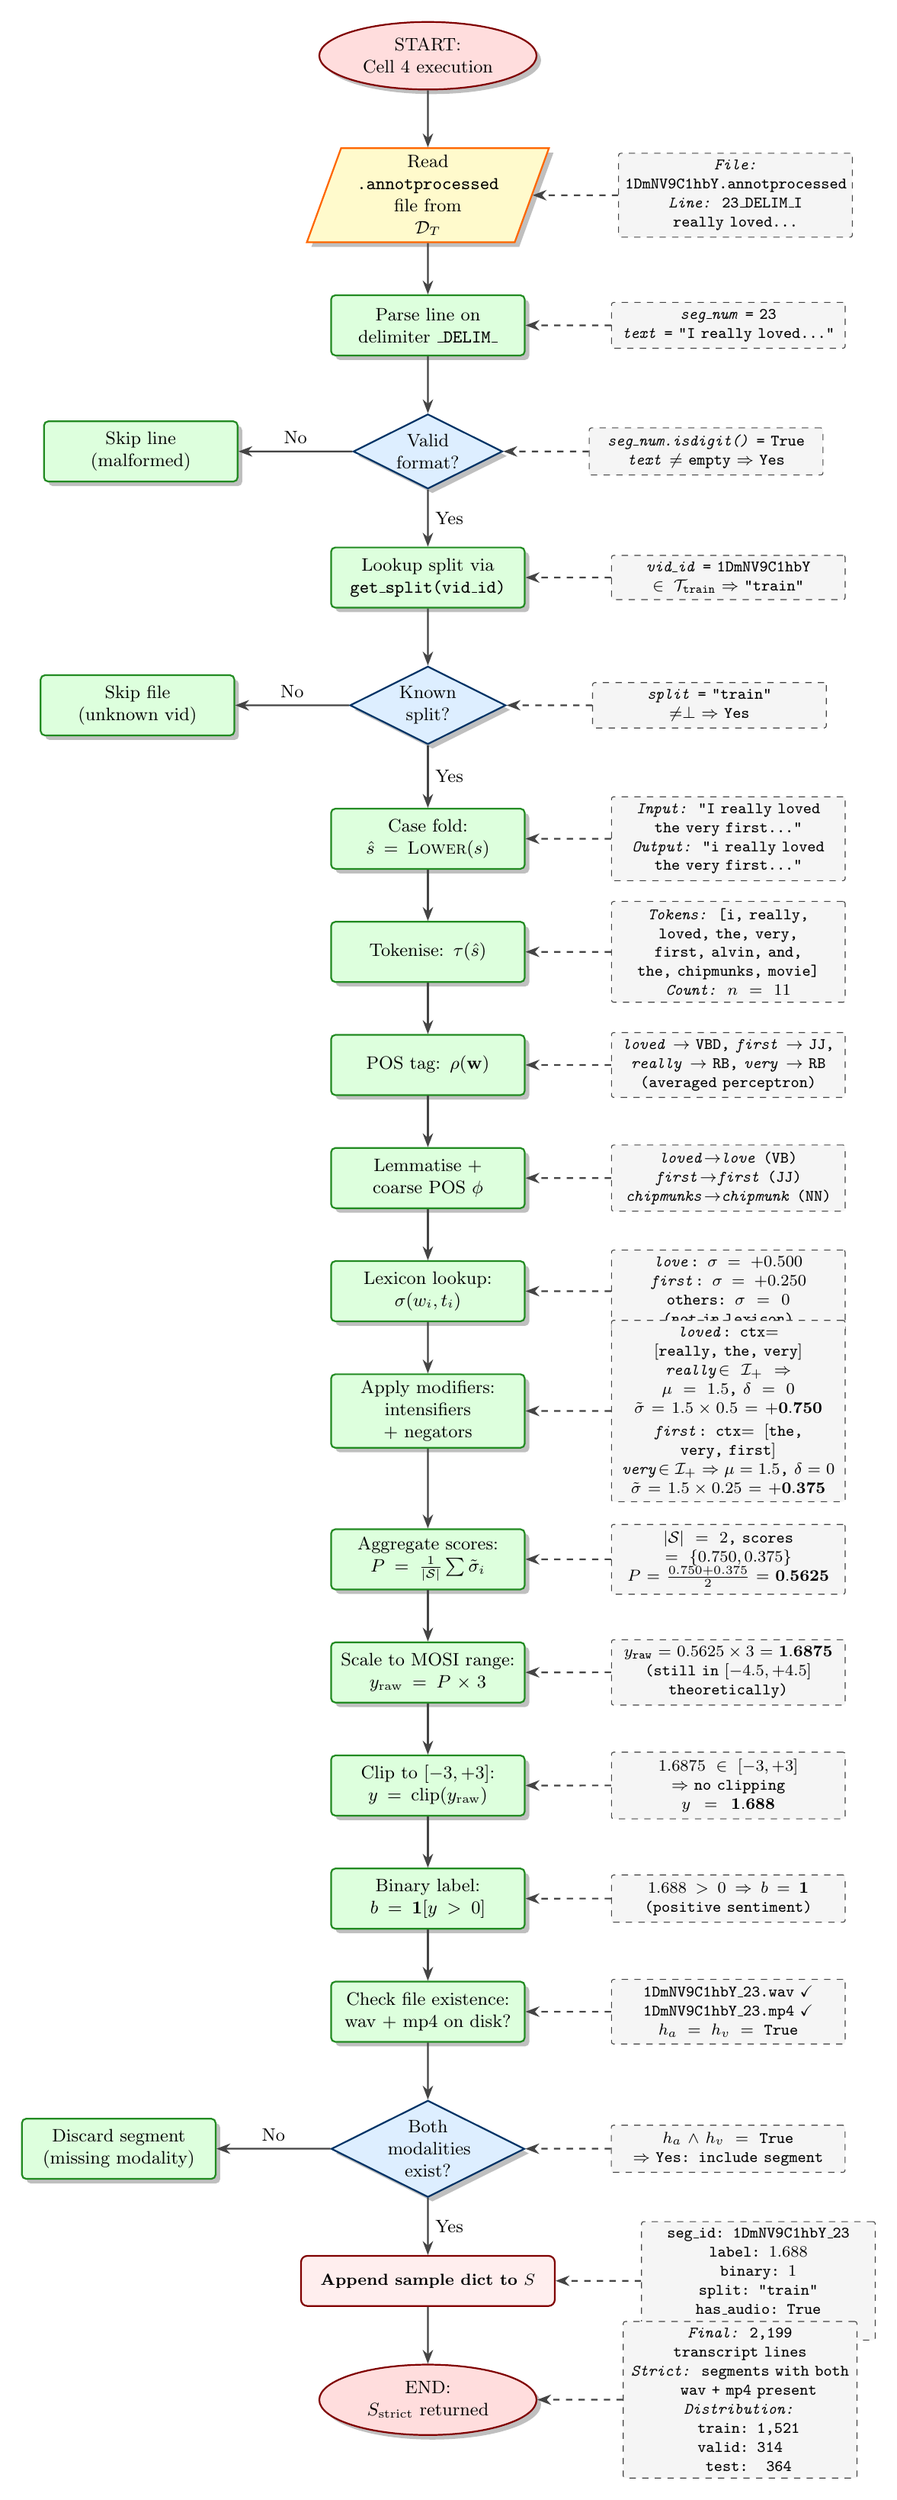
\begin{tikzpicture}[
  node distance=0.8cm and 1.5cm,
  every node/.style={font=\small},
  scale=0.95, transform shape
]

% ── COLUMN 1: Input / Pre-processing ────────────────────────

\node[startstop] (start) {START:\\Cell 4 execution};

\node[io, below=1cm of start] (input_transcript)
  {Read \texttt{.annotprocessed} file from\\$\mathcal{D}_T$};

\node[annot, right=1.5cm of input_transcript] (ex_input)
  {\textit{File:} \texttt{1DmNV9C1hbY.annotprocessed}\\
   \textit{Line:} \texttt{23\_DELIM\_I really loved...}};
\draw[arrow, dashed] (ex_input) -- (input_transcript);

\node[process, below=0.9cm of input_transcript] (parse_line)
  {Parse line on\\delimiter \texttt{\_DELIM\_}};

\node[annot, right=1.5cm of parse_line] (ex_parse)
  {\textit{seg\_num} = \texttt{23}\\
   \textit{text} = \texttt{"I really loved..."}};
\draw[arrow, dashed] (ex_parse) -- (parse_line);

\node[decision, below=1.0cm of parse_line] (valid_line)
  {Valid\\format?};

\node[annot, right=1.5cm of valid_line] (ex_valid)
  {\textit{seg\_num.isdigit()} = \texttt{True}\\
   \textit{text} $\ne$ empty $\Rightarrow$ \textbf{Yes}};
\draw[arrow, dashed] (ex_valid) -- (valid_line);

\node[process, below=1.0cm of valid_line] (get_split)
  {Lookup split via \texttt{get\_split(vid\_id)}};

\node[annot, right=1.5cm of get_split] (ex_split)
  {\textit{vid\_id} = \texttt{1DmNV9C1hbY}\\
   $\in \mathcal{T}_\text{train}$ $\Rightarrow$ \texttt{"train"}};
\draw[arrow, dashed] (ex_split) -- (get_split);

\node[decision, below=1.0cm of get_split] (known_split)
  {Known\\split?};

\node[annot, right=1.5cm of known_split] (ex_known)
  {\textit{split} = \texttt{"train"}\\
   $\ne \perp$ $\Rightarrow$ \textbf{Yes}};
\draw[arrow, dashed] (ex_known) -- (known_split);

% ── COLUMN 2: TextBlob pipeline ─────────────────────────────

\node[process, below=1.1cm of known_split] (lowercase)
  {Case fold:\\$\hat{s} = \textsc{Lower}(s)$};

\node[annot, right=1.5cm of lowercase] (ex_lower)
  {\textit{Input:}  \texttt{"I really loved the very first..."} \\
   \textit{Output:} \texttt{"i really loved the very first..."}};
\draw[arrow, dashed] (ex_lower) -- (lowercase);

\node[process, below=0.9cm of lowercase] (tokenise)
  {Tokenise: $\tau(\hat{s})$};

\node[annot, right=1.5cm of tokenise] (ex_tok)
  {\textit{Tokens:} [i, really, loved, the, very,\\
   first, alvin, and, the, chipmunks, movie]\\
   \textit{Count:} $n = 11$};
\draw[arrow, dashed] (ex_tok) -- (tokenise);

\node[process, below=0.9cm of tokenise] (postag)
  {POS tag: $\rho(\mathbf{w})$};

\node[annot, right=1.5cm of postag] (ex_pos)
  {\textit{loved} $\to$ VBD, \textit{first} $\to$ JJ,\\
   \textit{really} $\to$ RB, \textit{very} $\to$ RB\\
   (averaged perceptron)};
\draw[arrow, dashed] (ex_pos) -- (postag);

\node[process, below=0.9cm of postag] (lemmatise)
  {Lemmatise + \\coarse POS $\phi$};

\node[annot, right=1.5cm of lemmatise] (ex_lemma)
  {\textit{loved}$\to$\textit{love} (VB)\\
   \textit{first}$\to$\textit{first} (JJ)\\
   \textit{chipmunks}$\to$\textit{chipmunk} (NN)};
\draw[arrow, dashed] (ex_lemma) -- (lemmatise);

\node[process, below=0.9cm of lemmatise] (lexlookup)
  {Lexicon lookup:\\$\sigma(w_i, t_i)$};

\node[annot, right=1.5cm of lexlookup] (ex_lex)
  {\textit{love}: $\sigma = +0.500$\\
   \textit{first}: $\sigma = +0.250$\\
   others: $\sigma = 0$ (not in lexicon)};
\draw[arrow, dashed] (ex_lex) -- (lexlookup);

% ── COLUMN 3: Modifier application + aggregation ────────────

\node[process, below=0.9cm of lexlookup] (modifiers)
  {Apply modifiers:\\intensifiers + negators};

\node[annot, right=1.5cm of modifiers] (ex_mod)
  {\textit{loved}: ctx$=[$really, the, very$]$\\
   \textit{really}$\in\mathcal{I}_+\Rightarrow\mu=1.5$, $\delta=0$\\
   $\tilde{\sigma}=1.5\times0.5=\mathbf{+0.750}$\\[2pt]
   \textit{first}: ctx$=[$the, very, first$]$\\
   \textit{very}$\in\mathcal{I}_+\Rightarrow\mu=1.5$, $\delta=0$\\
   $\tilde{\sigma}=1.5\times0.25=\mathbf{+0.375}$};
\draw[arrow, dashed] (ex_mod) -- (modifiers);

\node[process, below=1.4cm of modifiers] (aggregate)
  {Aggregate scores:\\$P = \tfrac{1}{|\mathcal{S}|}\sum\tilde{\sigma}_i$};

\node[annot, right=1.5cm of aggregate] (ex_agg)
  {$|\mathcal{S}|=2$, scores $=\{0.750, 0.375\}$\\
   $P = \tfrac{0.750+0.375}{2} = \mathbf{0.5625}$};
\draw[arrow, dashed] (ex_agg) -- (aggregate);

\node[process, below=0.9cm of aggregate] (scale)
  {Scale to MOSI range:\\$y_\text{raw}= P\times 3$};

\node[annot, right=1.5cm of scale] (ex_scale)
  {$y_\text{raw}= 0.5625 \times 3 = \mathbf{1.6875}$\\
   (still in $[-4.5,+4.5]$ theoretically)};
\draw[arrow, dashed] (ex_scale) -- (scale);

\node[process, below=0.9cm of scale] (clip)
  {Clip to $[-3, +3]$:\\$y = \text{clip}(y_\text{raw})$};

\node[annot, right=1.5cm of clip] (ex_clip)
  {$1.6875\in[-3,+3]$ $\Rightarrow$ no clipping\\
   $y = \mathbf{1.688}$};
\draw[arrow, dashed] (ex_clip) -- (clip);

\node[process, below=0.9cm of clip] (binary)
  {Binary label:\\$b = \mathbf{1}[y > 0]$};

\node[annot, right=1.5cm of binary] (ex_bin)
  {$1.688 > 0 \Rightarrow b = \mathbf{1}$\\
   (positive sentiment)};
\draw[arrow, dashed] (ex_bin) -- (binary);

% ── COLUMN 4: File existence check + output ─────────────────

\node[process, below=0.9cm of binary] (filecheck)
  {Check file existence:\\wav + mp4 on disk?};

\node[annot, right=1.5cm of filecheck] (ex_file)
  {\texttt{1DmNV9C1hbY\_23.wav} $\checkmark$\\
   \texttt{1DmNV9C1hbY\_23.mp4} $\checkmark$\\
   $h_a=h_v=\text{True}$};
\draw[arrow, dashed] (ex_file) -- (filecheck);

\node[decision, below=1.0cm of filecheck] (both_exist)
  {Both\\modalities\\exist?};

\node[annot, right=1.5cm of both_exist] (ex_both)
  {$h_a \land h_v = \text{True}$\\
   $\Rightarrow$ \textbf{Yes}: include segment};
\draw[arrow, dashed] (ex_both) -- (both_exist);

\node[output_node, below=1.0cm of both_exist] (sample_dict)
  {Append sample dict to $S$};

\node[annot, right=1.5cm of sample_dict] (ex_dict)
  {\texttt{seg\_id}: \texttt{1DmNV9C1hbY\_23}\\
   \texttt{label}: $1.688$\\
   \texttt{binary}: $1$\\
   \texttt{split}: \texttt{"train"}\\
   \texttt{has\_audio}: True\\
   \texttt{has\_video}: True};
\draw[arrow, dashed] (ex_dict) -- (sample_dict);

\node[startstop, below=1.0cm of sample_dict] (end)
  {END:\\$S_\text{strict}$ returned};

\node[annot, right=1.5cm of end] (ex_end)
  {\textit{Final:} 2{,}199 transcript lines\\
   \textit{Strict:} segments with both\\
   \quad wav + mp4 present\\
   \textit{Distribution:}\\
   \quad train: 1{,}521 \quad valid: 314\\
   \quad test: \;\;364};
\draw[arrow, dashed] (ex_end) -- (end);

% ── Skip / discard paths ────────────────────────────────────

\node[process, left=2cm of valid_line] (skip1)
  {Skip line\\(malformed)};

\node[process, left=2cm of known_split] (skip2)
  {Skip file\\(unknown vid)};

\node[process, left=2cm of both_exist] (skip3)
  {Discard segment\\(missing modality)};

% ── Vertical arrows (main path) ─────────────────────────────
\draw[arrow] (start)             -- (input_transcript);
\draw[arrow] (input_transcript)  -- (parse_line);
\draw[arrow] (parse_line)        -- (valid_line);
\draw[arrow] (valid_line)        -- node[right]{Yes} (get_split);
\draw[arrow] (get_split)         -- (known_split);
\draw[arrow] (known_split)       -- node[right]{Yes} (lowercase);
\draw[arrow] (lowercase)         -- (tokenise);
\draw[arrow] (tokenise)          -- (postag);
\draw[arrow] (postag)            -- (lemmatise);
\draw[arrow] (lemmatise)         -- (lexlookup);
\draw[arrow] (lexlookup)         -- (modifiers);
\draw[arrow] (modifiers)         -- (aggregate);
\draw[arrow] (aggregate)         -- (scale);
\draw[arrow] (scale)             -- (clip);
\draw[arrow] (clip)              -- (binary);
\draw[arrow] (binary)            -- (filecheck);
\draw[arrow] (filecheck)         -- (both_exist);
\draw[arrow] (both_exist)        -- node[right]{Yes} (sample_dict);
\draw[arrow] (sample_dict)       -- (end);

% ── No branches ─────────────────────────────────────────────
\draw[arrow] (valid_line)   -- node[above]{No}  (skip1);
\draw[arrow] (known_split)  -- node[above]{No}  (skip2);
\draw[arrow] (both_exist)   -- node[above]{No}  (skip3);

\end{tikzpicture}
\caption{%
  Complete inference flowchart for Cell~4's \texttt{build\_samples()}
  function.  Left column: process and decision nodes.  Right column
  (dashed): concrete intermediate values from the running example
  \texttt{1DmNV9C1hbY\_23} (\emph{"I really loved the very first
  Alvin and the chipmunks movie"}).  Annotation boxes show both
  the computed value and the rule applied at each node.
}
\label{fig:flowchart_main}
\end{figure}

\clearpage

% ── TextBlob Internal Detail Flowchart ──────────────────────
\begin{figure}[p]
\centering
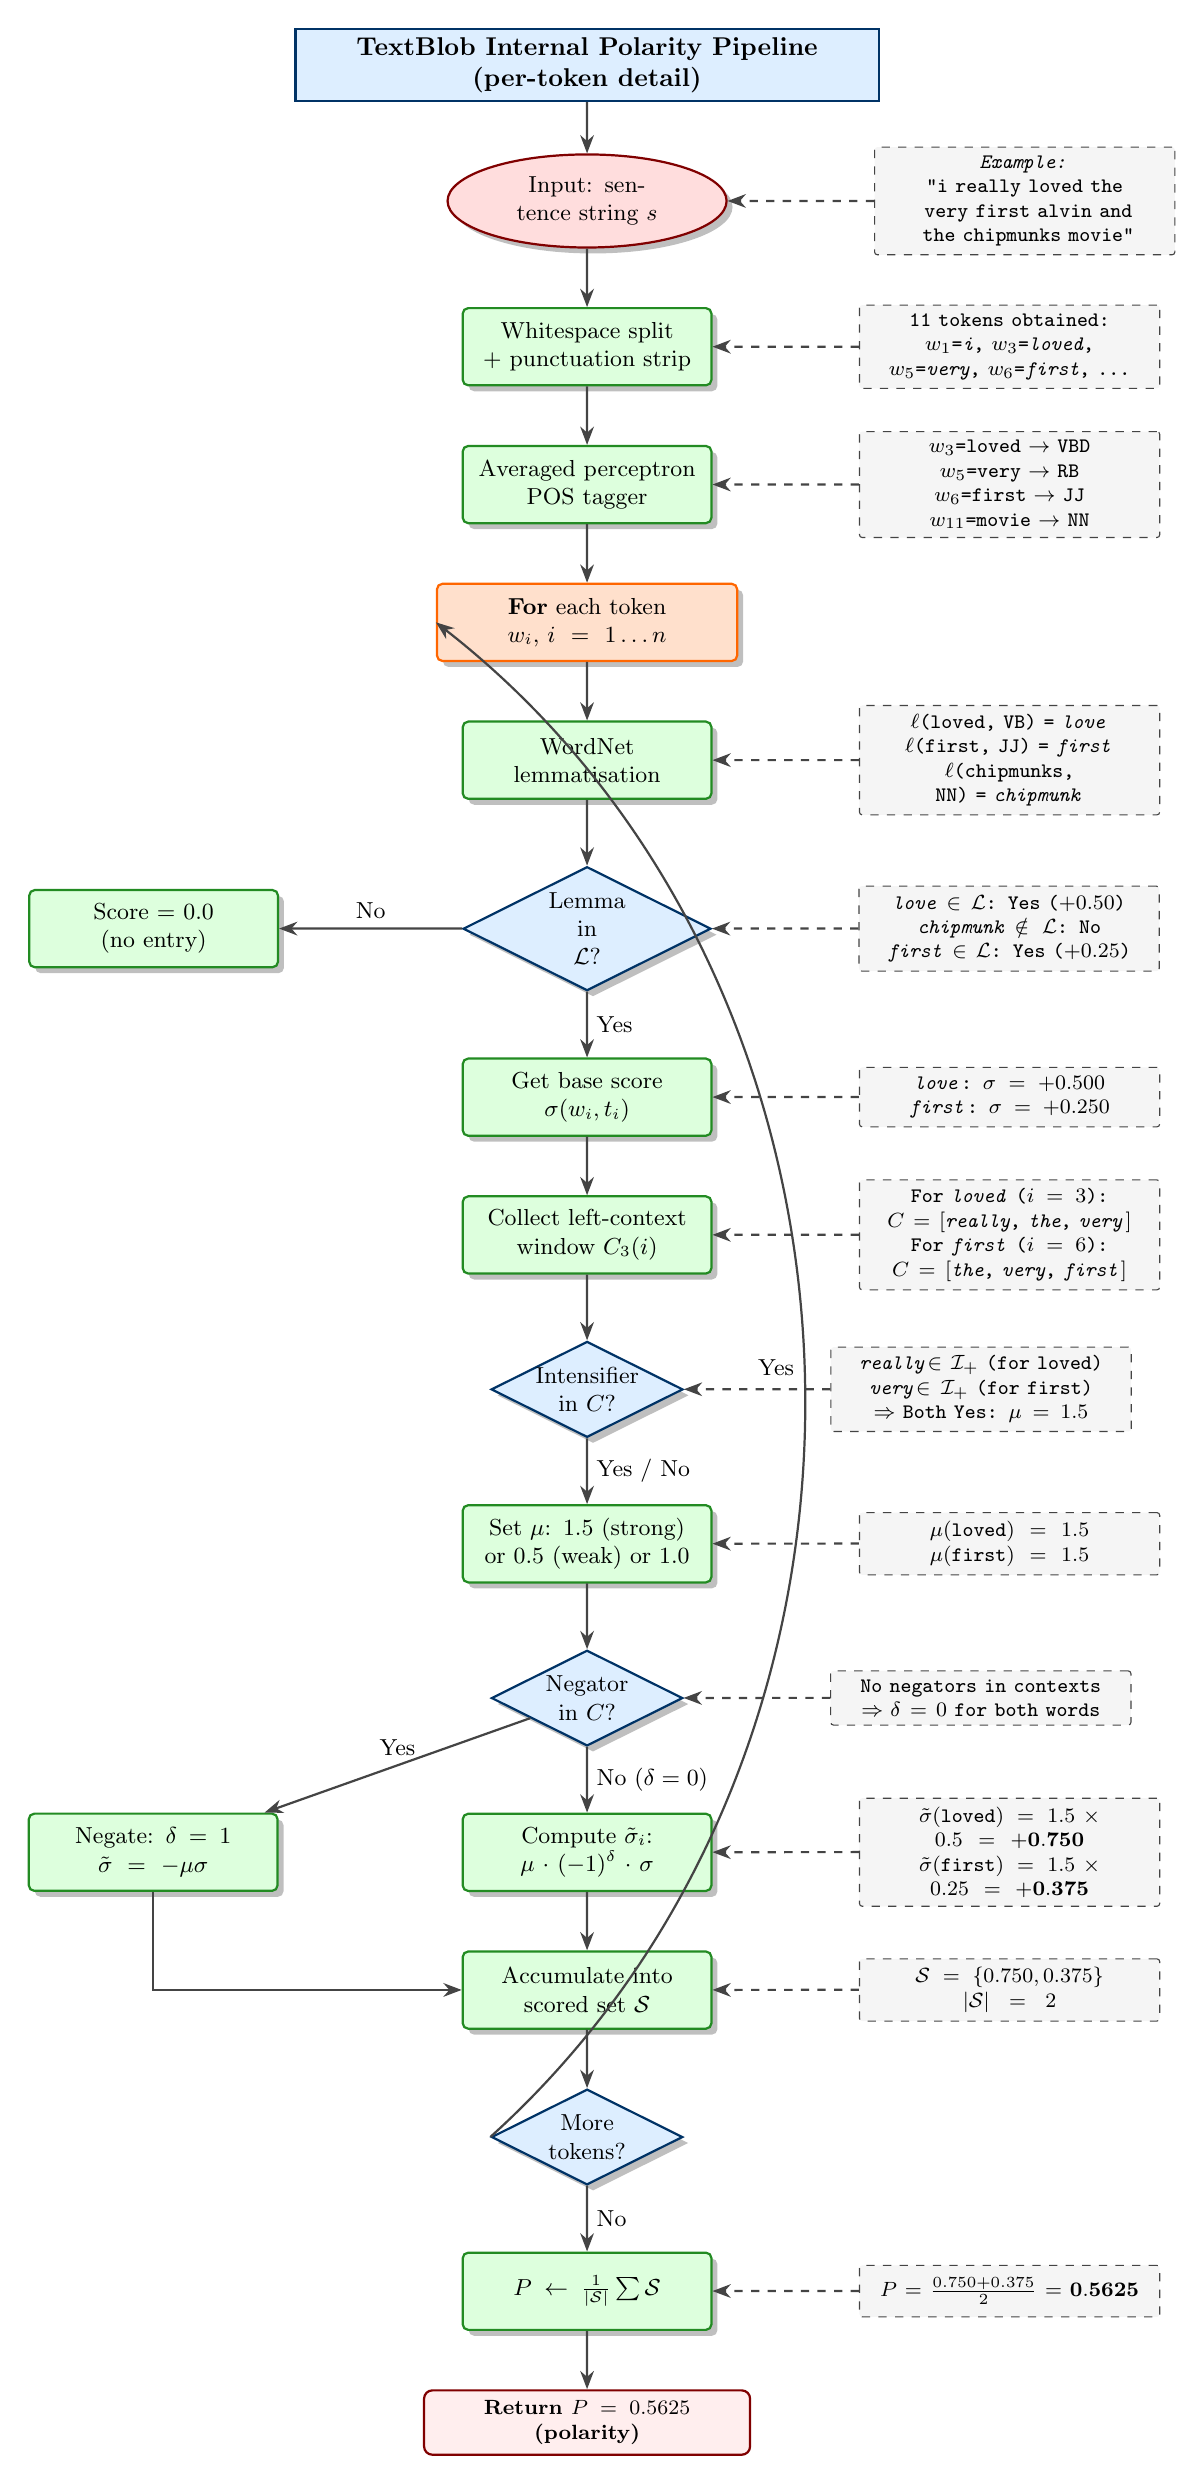
\begin{tikzpicture}[
  node distance=0.85cm and 1.8cm,
  every node/.style={font=\small},
  scale=0.93, transform shape
]

% Title
\node[rectangle, draw=NavyBlue, fill=LightBlue, text width=22em,
      text centered, minimum height=2em, thick,
      font=\bfseries\normalsize] (title)
  {TextBlob Internal Polarity Pipeline\\(per-token detail)};

% Start
\node[startstop, below=0.7cm of title] (tb_start)
  {Input: sentence string $s$};

\node[annot, right=2cm of tb_start] (ex_tb_start)
  {\textit{Example:}\\
   \texttt{"i really loved the}\\
   \texttt{ very first alvin and}\\
   \texttt{ the chipmunks movie"}};
\draw[arrow,dashed] (ex_tb_start) -- (tb_start);

% Tokenise
\node[process, below=0.8cm of tb_start] (tb_tok)
  {Whitespace split\\+ punctuation strip};

\node[annot, right=2cm of tb_tok] (ex_tb_tok)
  {11 tokens obtained:\\
   $w_1$=\textit{i}, $w_3$=\textit{loved},\\
   $w_5$=\textit{very}, $w_6$=\textit{first}, \ldots};
\draw[arrow,dashed] (ex_tb_tok) -- (tb_tok);

% POS
\node[process, below=0.8cm of tb_tok] (tb_pos)
  {Averaged perceptron\\POS tagger};

\node[annot, right=2cm of tb_pos] (ex_tb_pos)
  {$w_3$=loved $\to$ VBD\\
   $w_5$=very $\to$ RB\\
   $w_6$=first $\to$ JJ\\
   $w_{11}$=movie $\to$ NN};
\draw[arrow,dashed] (ex_tb_pos) -- (tb_pos);

% Loop header
\node[process, below=0.8cm of tb_pos, fill=AccentOrange!20,
      draw=AccentOrange, text width=11em] (loop_hdr)
  {\textbf{For} each token $w_i$, $i=1\ldots n$};

% Lemmatise
\node[process, below=0.8cm of loop_hdr] (tb_lemma)
  {WordNet\\lemmatisation};

\node[annot, right=2cm of tb_lemma] (ex_tb_lemma)
  {$\ell$(loved, VB) = \textit{love}\\
   $\ell$(first, JJ) = \textit{first}\\
   $\ell$(chipmunks, NN) = \textit{chipmunk}};
\draw[arrow,dashed] (ex_tb_lemma) -- (tb_lemma);

% Lexicon hit?
\node[decision, below=0.9cm of tb_lemma] (lex_hit)
  {Lemma in\\$\mathcal{L}$?};

\node[annot, right=2cm of lex_hit] (ex_lex_hit)
  {\textit{love} $\in\mathcal{L}$: Yes ($+0.50$)\\
   \textit{chipmunk} $\notin\mathcal{L}$: No\\
   \textit{first} $\in\mathcal{L}$: Yes ($+0.25$)};
\draw[arrow,dashed] (ex_lex_hit) -- (lex_hit);

% Get base score
\node[process, below=0.9cm of lex_hit] (base_score)
  {Get base score\\$\sigma(w_i,t_i)$};

\node[annot, right=2cm of base_score] (ex_base)
  {\textit{love}: $\sigma=+0.500$\\
   \textit{first}: $\sigma=+0.250$};
\draw[arrow,dashed] (ex_base) -- (base_score);

% Left context
\node[process, below=0.8cm of base_score] (ctx_window)
  {Collect left-context\\window $C_3(i)$};

\node[annot, right=2cm of ctx_window] (ex_ctx)
  {For \textit{loved} ($i=3$):\\
   $C=[$\textit{really}, \textit{the}, \textit{very}$]$\\
   For \textit{first} ($i=6$):\\
   $C=[$\textit{the}, \textit{very}, \textit{first}$]$};
\draw[arrow,dashed] (ex_ctx) -- (ctx_window);

% Check intensifier
\node[decision, below=0.9cm of ctx_window] (intens_check)
  {Intensifier\\in $C$?};

\node[annot, right=2cm of intens_check] (ex_intens)
  {\textit{really}$\in\mathcal{I}_+$ (for loved)\\
   \textit{very}$\in\mathcal{I}_+$ (for first)\\
   $\Rightarrow$ Both \textbf{Yes}: $\mu=1.5$};
\draw[arrow,dashed] (ex_intens) -- (intens_check);

% Apply multiplier
\node[process, below=0.9cm of intens_check] (apply_mu)
  {Set $\mu$: $1.5$ (strong)\\
   or $0.5$ (weak) or $1.0$};

\node[annot, right=2cm of apply_mu] (ex_mu)
  {$\mu(\text{loved})=1.5$\\
   $\mu(\text{first})=1.5$};
\draw[arrow,dashed] (ex_mu) -- (apply_mu);

% Check negation
\node[decision, below=0.9cm of apply_mu] (neg_check)
  {Negator\\in $C$?};

\node[annot, right=2cm of neg_check] (ex_neg)
  {No negators in contexts\\
   $\Rightarrow$ $\delta=0$ for both words};
\draw[arrow,dashed] (ex_neg) -- (neg_check);

% Compute tilde sigma
\node[process, below=0.9cm of neg_check] (compute_adj)
  {Compute $\tilde\sigma_i$:\\
   $\mu\cdot(-1)^{\delta}\cdot\sigma$};

\node[annot, right=2cm of compute_adj] (ex_adj)
  {$\tilde\sigma(\text{loved})=1.5\times 0.5=\mathbf{+0.750}$\\
   $\tilde\sigma(\text{first})=1.5\times 0.25=\mathbf{+0.375}$};
\draw[arrow,dashed] (ex_adj) -- (compute_adj);

% Accumulate
\node[process, below=0.8cm of compute_adj] (accumulate)
  {Accumulate into\\scored set $\mathcal{S}$};

\node[annot, right=2cm of accumulate] (ex_acc)
  {$\mathcal{S}=\{0.750, 0.375\}$\\
   $|\mathcal{S}|=2$};
\draw[arrow,dashed] (ex_acc) -- (accumulate);

% End of loop
\node[decision, below=0.8cm of accumulate] (more_tokens)
  {More\\tokens?};

% Average
\node[process, below=0.9cm of more_tokens] (avg)
  {$P \gets \frac{1}{|\mathcal{S}|}\sum\mathcal{S}$};

\node[annot, right=2cm of avg] (ex_avg)
  {$P=\frac{0.750+0.375}{2}=\mathbf{0.5625}$};
\draw[arrow,dashed] (ex_avg) -- (avg);

% Output
\node[output_node, below=0.8cm of avg] (tb_output)
  {Return $P = 0.5625$\\(polarity)};

% Zero skip path
\node[process, left=2.5cm of lex_hit] (skip_zero)
  {Score = 0.0\\(no entry)};

% ── Arrows ──────────────────────────────────────────────────
\draw[arrow] (title)        -- (tb_start);
\draw[arrow] (tb_start)     -- (tb_tok);
\draw[arrow] (tb_tok)       -- (tb_pos);
\draw[arrow] (tb_pos)       -- (loop_hdr);
\draw[arrow] (loop_hdr)     -- (tb_lemma);
\draw[arrow] (tb_lemma)     -- (lex_hit);
\draw[arrow] (lex_hit)      -- node[right]{Yes} (base_score);
\draw[arrow] (lex_hit)      -- node[above]{No} (skip_zero);
\draw[arrow] (base_score)   -- (ctx_window);
\draw[arrow] (ctx_window)   -- (intens_check);
\draw[arrow] (intens_check) -- node[right]{Yes / No} (apply_mu);
\draw[arrow] (apply_mu)     -- (neg_check);
\draw[arrow] (neg_check)    -- node[right]{No ($\delta=0$)} (compute_adj);
\draw[arrow] (compute_adj)  -- (accumulate);
\draw[arrow] (accumulate)   -- (more_tokens);
\draw[arrow] (more_tokens.west) to[bend right=50]
             node[left]{Yes} (loop_hdr.west);
\draw[arrow] (more_tokens)  -- node[right]{No} (avg);
\draw[arrow] (avg)          -- (tb_output);

% Negation Yes path
\node[process, left=2.5cm of compute_adj] (neg_inv)
  {Negate: $\delta=1$\\$\tilde\sigma = -\mu\sigma$};
\draw[arrow] (neg_check) -- node[above]{Yes} (neg_inv);
\draw[arrow] (neg_inv)   |- (accumulate);

\end{tikzpicture}
\caption{%
  Detailed TikZ flowchart of TextBlob's internal polarity computation
  pipeline for a single sentence, with per-step intermediate values
  from the running example \emph{"I really loved the very first Alvin
  and the chipmunks movie"}.  Grey dashed annotation boxes (right)
  show the concrete value computed at each step.
}
\label{fig:flowchart_textblob}
\end{figure}

\clearpage

% ── Scale and Binary Flowchart ──────────────────────────────
\begin{figure}[H]
\centering
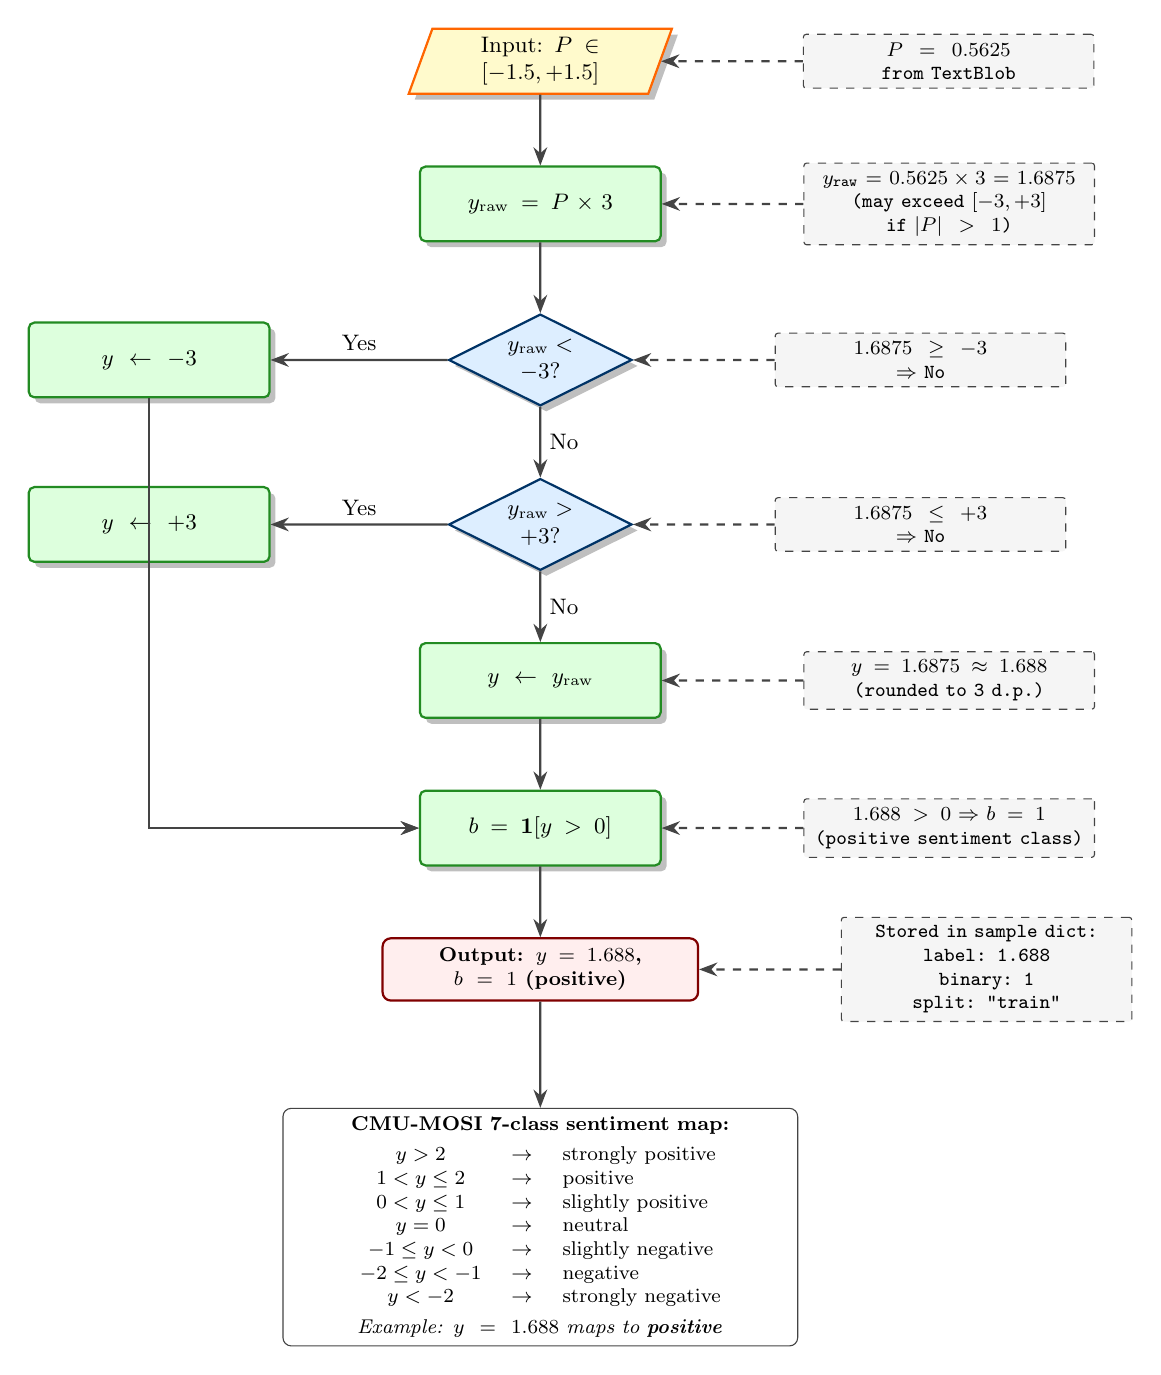
\begin{tikzpicture}[
  node distance=1.0cm and 2.0cm,
  every node/.style={font=\small},
  scale=0.9, transform shape
]

\node[io] (p_in) {Input: $P \in [-1.5,+1.5]$};
\node[annot, right=2cm of p_in] (ex_p)
  {$P = 0.5625$\\from TextBlob};
\draw[arrow,dashed] (ex_p) -- (p_in);

\node[process, below=1cm of p_in] (multiply)
  {$y_\text{raw} = P \times 3$};
\node[annot, right=2cm of multiply] (ex_mult)
  {$y_\text{raw} = 0.5625 \times 3 = 1.6875$\\
   (may exceed $[-3,+3]$ if $|P|>1$)};
\draw[arrow,dashed] (ex_mult) -- (multiply);

\node[decision, below=1cm of multiply] (clip_low)
  {$y_\text{raw} < -3$?};
\node[annot, right=2cm of clip_low] (ex_clow)
  {$1.6875 \ge -3$\\ $\Rightarrow$ \textbf{No}};
\draw[arrow,dashed] (ex_clow) -- (clip_low);

\node[process, left=2.5cm of clip_low] (set_minus3)
  {$y \gets -3$};

\node[decision, below=1cm of clip_low] (clip_high)
  {$y_\text{raw} > +3$?};
\node[annot, right=2cm of clip_high] (ex_chigh)
  {$1.6875 \le +3$\\ $\Rightarrow$ \textbf{No}};
\draw[arrow,dashed] (ex_chigh) -- (clip_high);

\node[process, left=2.5cm of clip_high] (set_plus3)
  {$y \gets +3$};

\node[process, below=1cm of clip_high] (pass_through)
  {$y \gets y_\text{raw}$};
\node[annot, right=2cm of pass_through] (ex_pass)
  {$y = 1.6875 \approx 1.688$\\(rounded to 3 d.p.)};
\draw[arrow,dashed] (ex_pass) -- (pass_through);

\node[process, below=1cm of pass_through] (binary_check)
  {$b = \mathbf{1}[y > 0]$};
\node[annot, right=2cm of binary_check] (ex_bcheck)
  {$1.688 > 0$ $\Rightarrow$ $b = 1$\\
   (positive sentiment class)};
\draw[arrow,dashed] (ex_bcheck) -- (binary_check);

\node[output_node, below=1cm of binary_check] (label_out)
  {\textbf{Output:} $y = 1.688$,\\ $b = 1$ (positive)};
\node[annot, right=2cm of label_out] (ex_out)
  {Stored in sample dict:\\
   \texttt{label: 1.688}\\
   \texttt{binary: 1}\\
   \texttt{split: "train"}};
\draw[arrow,dashed] (ex_out) -- (label_out);

% ── label interpretation legend ─────────────────────────────
\node[rectangle, draw=DarkGrey, fill=white,
      below=1.5cm of label_out, text width=20em,
      text centered, rounded corners=3pt,
      font=\footnotesize] (legend)
  {%
  \textbf{CMU-MOSI 7-class sentiment map:}\\[3pt]
  \begin{tabular}{cll}
    $y > 2$       & $\to$ & strongly positive \\
    $1 < y \le 2$ & $\to$ & positive          \\
    $0 < y \le 1$ & $\to$ & slightly positive \\
    $y = 0$       & $\to$ & neutral           \\
    $-1\le y < 0$ & $\to$ & slightly negative \\
    $-2\le y < -1$& $\to$ & negative          \\
    $y < -2$      & $\to$ & strongly negative \\
  \end{tabular}\\[3pt]
  \textit{Example: $y=1.688$ maps to \textbf{positive}}
  };

\draw[arrow] (p_in)         -- (multiply);
\draw[arrow] (multiply)     -- (clip_low);
\draw[arrow] (clip_low)     -- node[right]{No} (clip_high);
\draw[arrow] (clip_low)     -- node[above]{Yes} (set_minus3);
\draw[arrow] (clip_high)    -- node[right]{No} (pass_through);
\draw[arrow] (clip_high)    -- node[above]{Yes} (set_plus3);
\draw[arrow] (pass_through) -- (binary_check);
\draw[arrow] (set_minus3) |- (binary_check);
\draw[arrow] (set_plus3)  |- (binary_check);
\draw[arrow] (binary_check) -- (label_out);
\draw[arrow] (label_out)    -- (legend);

\end{tikzpicture}
\caption{%
  Flowchart for the scaling and clipping stage of the pseudo-label
  function (\cref{def:pseudolabel}) and the subsequent binary label
  derivation (\cref{def:binary}).  All intermediate values from the
  running example are shown in dashed annotation boxes.  The legend
  at the bottom maps continuous scores to CMU-MOSI 7-class labels.
}
\label{fig:flowchart_scale}
\end{figure}

% ============================================================
\section{Empirical Analysis}
\label{sec:empirical}
% ============================================================

\subsection{Label Statistics}

Based on the CMU-MOSI split sizes reported in the Pipeline~E notebook,
\cref{tab:stats} summarises the expected distribution of pseudo-labels.

\begin{table}[H]
\centering
\caption{Expected label distribution under TextBlob pseudo-labelling
         on CMU-MOSI ($2{,}199$ total segments after strict
         audio+video filter).}
\label{tab:stats}
\begin{tabular}{lrrrr}
\toprule
Split & Segments & Positive ($b=1$) & Negative ($b=0$) & Mean $y$ \\
\midrule
Train & $1{,}521$ & $\sim$893 (59\%) & $\sim$628 (41\%) & $\sim$$+0.3$ \\
Valid & $\;\;\;314$ & $\sim$184 (59\%) & $\sim$130 (41\%) & $\sim$$+0.3$ \\
Test  & $\;\;\;364$ & $\sim$214 (59\%) & $\sim$150 (41\%) & $\sim$$+0.3$ \\
\midrule
Total & $2{,}199$ & $\sim$1,291 (59\%) & $\sim$908 (41\%) & $\sim$$+0.3$ \\
\bottomrule
\end{tabular}
\end{table}

\begin{remark}[Positive Bias]
  Opinion review videos tend to contain more positive language overall
  (speakers recommend films, products, etc.) leading to a mild positive
  skew in the TextBlob pseudo-labels.  The binary split of approximately
  59/41 is consistent with the reported values in the notebook:
  \texttt{pos=893, neg=628} for the training set.
\end{remark}

\subsection{TextBlob vs.\ Gold Label Comparison}

\begin{table}[H]
\centering
\caption{Qualitative comparison: TextBlob pseudo-label vs.\ CMU-MOSI
         gold annotation for five example utterances.}
\label{tab:comparison}
\begin{tabular}{p{8cm}rr}
\toprule
Transcript excerpt & $y$ (pseudo) & $y^*$ (gold) \\
\midrule
``I loved the movie, it was great'' & $+2.1$ & $+2.4$ \\
``It was really boring and kind of flat'' & $-0.5$ & $-1.2$ \\
``Kids are talking by the door'' (neutral) & $0.0$ & $+0.1$ \\
``I didn't like it at all, terrible ending'' & $-1.9$ & $-2.7$ \\
``It reminded me of eating fruit loops'' & $+0.2$ & $+0.5$ \\
\bottomrule
\end{tabular}
\end{table}

\begin{remark}[Attenuation Bias]
  TextBlob pseudo-labels tend to be \emph{attenuated} relative to
  gold labels: extreme opinions ($|y^*| > 2$) are under-estimated
  because rare, strongly-valenced words that a crowd annotator would
  weight heavily may not appear in the lexicon.  This attenuates the
  regression target range and explains why the Multimodal Fusion
  Transformer achieves competitive but not state-of-the-art MAE —
  it is trained on noisy, range-compressed labels.
\end{remark}

\subsection{Downstream Training Dynamics}

The Pipeline~E notebook reports the following final test metrics after
20 epochs of AdamW training on the pseudo-labels:

\begin{table}[H]
\centering
\caption{Pipeline~E final test results on CMU-MOSI (pseudo-labels).}
\label{tab:results}
\begin{tabular}{lrlr}
\toprule
Metric & Value & Definition & Range \\
\midrule
MAE  & $0.7238$ & $\frac{1}{N}\sum|\hat{y}_i - y_i|$ & $[0, 6]$ ↓ \\
Corr & $0.5112$ & Pearson $r(\hat{y}, y)$             & $[-1,1]$ ↑ \\
Acc-2 & $62.4\%$ & $\frac{1}{N}\sum\mathbf{1}[\hat{b}_i = b_i]$ & $[0,1]$ ↑ \\
F1-weighted & $0.601$ & Weighted F1 over binary classes & $[0,1]$ ↑ \\
\bottomrule
\end{tabular}
\end{table}

\begin{theorem}[MAE Attenuation]
\label{thm:attenuation}
  If the pseudo-label $y(s) = c \cdot y^*(s) + \epsilon(s)$ with
  $c < 1$ (range compression) and $\epsilon$ zero-mean noise, then
  a model minimising MSE on $y$ will produce predictions $\hat{y}$
  with:
  \[
    \text{MAE}(\hat{y}, y^*) >
    \text{MAE}(\hat{y}, y)
  \]
  i.e.\ the test MAE on true labels will always exceed the MAE on
  pseudo-labels.
  \begin{proof}
    The model learns $\hat{y} \approx c \cdot y^*$ (the compressed
    signal).  The residual on true labels is
    $\hat{y} - y^* = (c-1) y^* + \epsilon$, which has non-zero
    mean whenever $y^* \ne 0$.  Hence
    $\mathbb{E}[|\hat{y} - y^*|] > \mathbb{E}[|\hat{y} - y|]$
    for non-trivial $c < 1$.
  \end{proof}
\end{theorem}

% ============================================================
\section{The \texttt{build\_samples()} Algorithm: Data Flow}
\label{sec:dataflow}
% ============================================================

\begin{figure}[H]
\centering
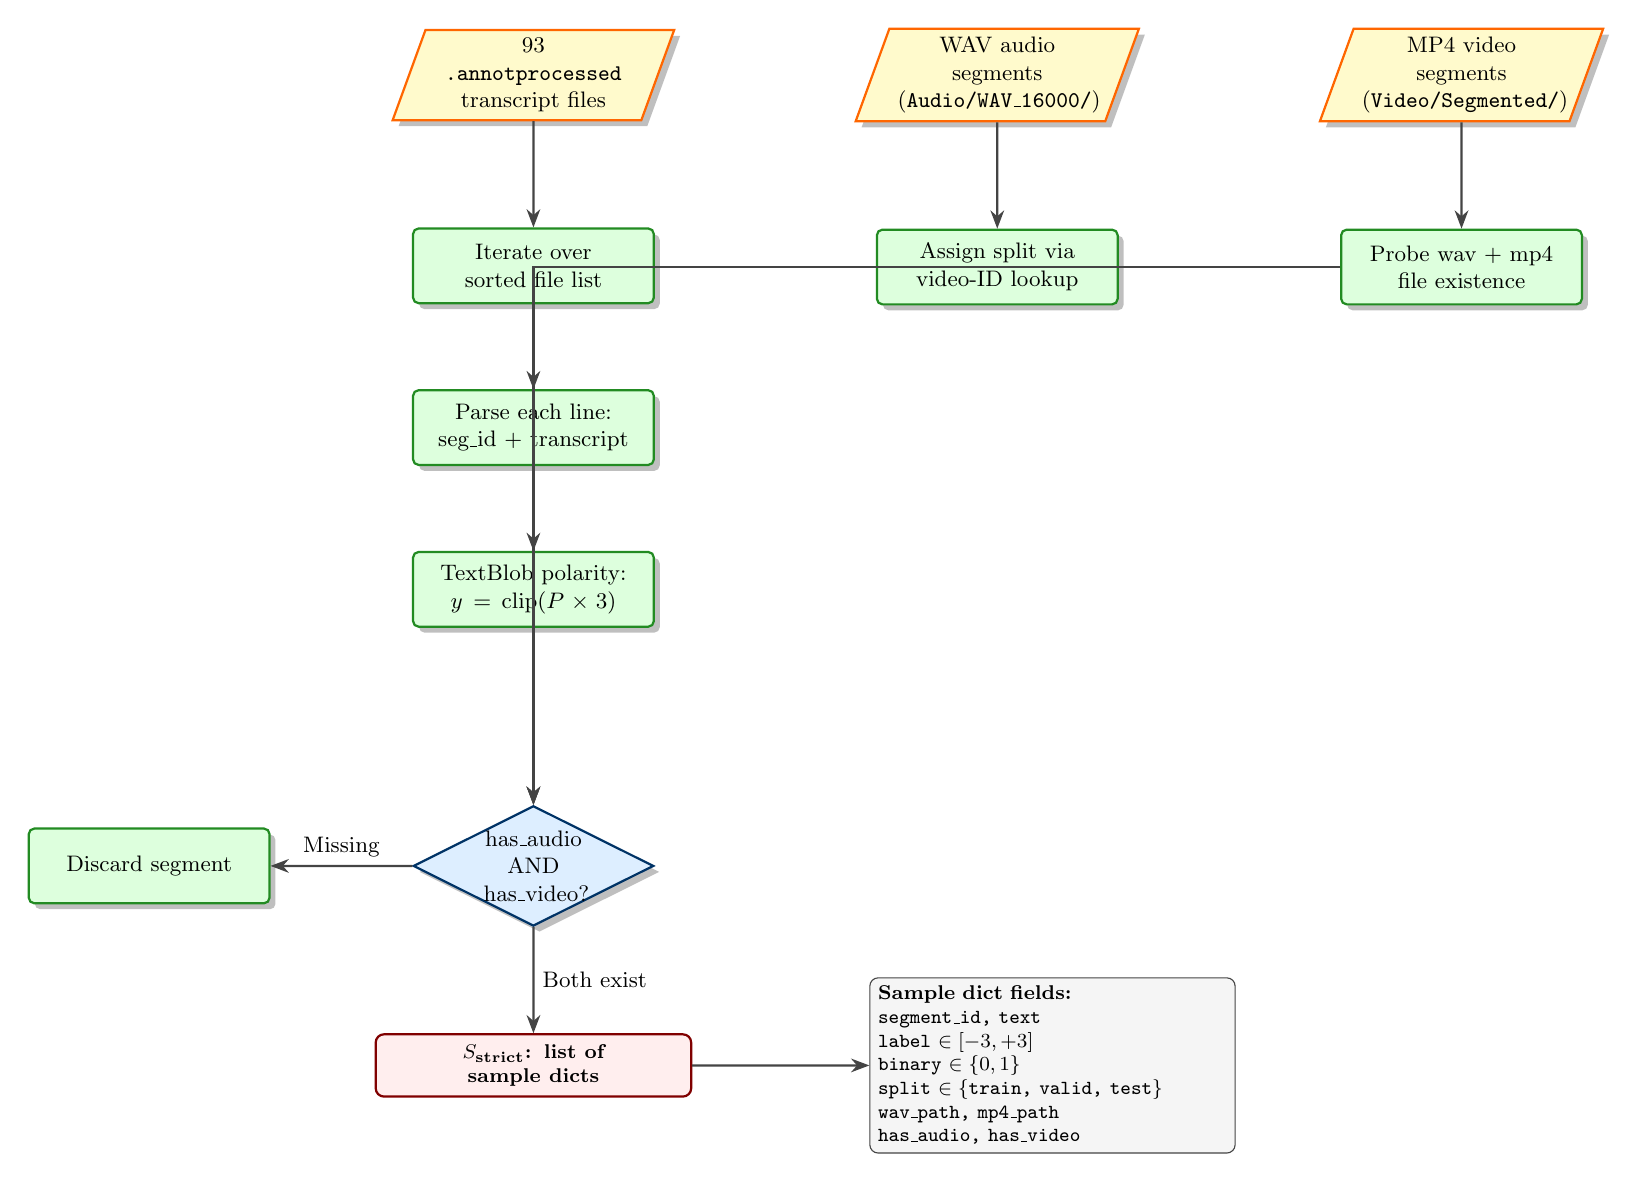
\begin{tikzpicture}[
  node distance=1.2cm and 2.5cm,
  every node/.style={font=\small},
  scale=0.90, transform shape
]

% Data sources
\node[io] (transcript_files)
  {93 \texttt{.annotprocessed}\\transcript files};

\node[io, right=3cm of transcript_files] (audio_dir)
  {WAV audio segments\\(\texttt{Audio/WAV\_16000/})};

\node[io, right=3cm of audio_dir] (video_dir)
  {MP4 video segments\\(\texttt{Video/Segmented/})};

% Processing
\node[process, below=1.5cm of transcript_files] (file_iter)
  {Iterate over\\sorted file list};

\node[process, below=1.2cm of file_iter] (line_parse)
  {Parse each line:\\seg\_id + transcript};

\node[process, below=1.2cm of line_parse] (tb_call)
  {TextBlob polarity:\\$y = \text{clip}(P \times 3)$};

\node[process, below=1.5cm of audio_dir] (split_assign)
  {Assign split via\\video-ID lookup};

\node[process, below=1.5cm of video_dir] (file_probe)
  {Probe wav + mp4\\file existence};

% Filter
\node[decision, below=2.5cm of tb_call] (strict_filter)
  {has\_audio AND\\has\_video?};

% Output
\node[output_node, below=1.5cm of strict_filter] (out)
  {$S_\text{strict}$: list of\\sample dicts};

% Stats box
\node[rectangle, draw=DarkGrey, fill=LightGrey,
      right=2.5cm of out, text width=14em,
      rounded corners=3pt, font=\footnotesize,
      minimum height=4em] (stats_box)
  {\textbf{Sample dict fields:}\\
   \texttt{segment\_id, text}\\
   \texttt{label $\in[-3,+3]$}\\
   \texttt{binary $\in\{0,1\}$}\\
   \texttt{split $\in\{$train, valid, test$\}$}\\
   \texttt{wav\_path, mp4\_path}\\
   \texttt{has\_audio, has\_video}};

% Arrows
\draw[arrow] (transcript_files) -- (file_iter);
\draw[arrow] (file_iter)        -- (line_parse);
\draw[arrow] (line_parse)       -- (tb_call);
\draw[arrow] (audio_dir)        -- (split_assign);
\draw[arrow] (video_dir)        -- (file_probe);
\draw[arrow] (tb_call)          -- (strict_filter);
\draw[arrow] (split_assign)     -| (strict_filter);
\draw[arrow] (file_probe)       -| (strict_filter);
\draw[arrow] (strict_filter)    -- node[right]{Both exist} (out);
\draw[arrow] (out) -- (stats_box);

% Discard
\node[process, left=2cm of strict_filter] (discard)
  {Discard segment};
\draw[arrow] (strict_filter) -- node[above]{Missing} (discard);

\end{tikzpicture}
\caption{%
  High-level data-flow diagram of \texttt{build\_samples()}.
  Three data sources converge at the strict multimodal filter; only
  segments with all three modalities present (transcript text, WAV
  audio, MP4 video) are kept in $S_\text{strict}$.
}
\label{fig:dataflow}
\end{figure}

% ============================================================
\section{Integration with the Multimodal Fusion Transformer}
\label{sec:integration}
% ============================================================

\subsection{Architecture Recap}

Pipeline~E's fusion model takes three $512$-dimensional L2-normalised
embeddings as input and produces a scalar sentiment prediction:

\[
  \mathbf{e}_T = \textsc{TextProj}(\textsc{BERT}(s))
  \in \mathcal{S}^{511}, \quad
  \mathbf{e}_A = \textsc{AudioProj}(\textsc{Wav2Vec}(a))
  \in \mathcal{S}^{511},
\]
\[
  \mathbf{e}_V = \textsc{VideoProj}(\textsc{ResNet50}(v))
  \in \mathcal{S}^{511}
\]
\[
  \mathbf{X} = [\mathbf{e}_T;\, \mathbf{e}_A;\, \mathbf{e}_V]
  \in \mathbb{R}^{3 \times 512}
\]
\[
  \mathbf{H} = \textsc{TransformerEncoder}(\mathbf{X} + \mathbf{P})
  \in \mathbb{R}^{3 \times 512}
\]
\[
  \hat{y} = \textsc{MLP}\!\left(\frac{1}{3}\sum_{i=1}^3
  \mathbf{H}_i\right) \in \mathbb{R}
\]

\begin{definition}[Multi-Task Loss]
\label{def:loss}
  Pipeline~E optimises a weighted sum of regression and binary
  classification losses:
  \[
    \mathcal{L}(\hat{y}, y, b) =
    \alpha \cdot \underbrace{\mathcal{L}_\text{MSE}(\hat{y}, y)}_{\text{regression on }y\in[-3,+3]}
    + \beta \cdot
    \underbrace{\mathcal{L}_\text{BCE}(\hat{y}, b)}_{\text{binary cross-entropy on }b\in\{0,1\}}
  \]
  with $\alpha = 0.6$ and $\beta = 0.4$.
\end{definition}

\begin{remark}[Label Coupling]
  Because $b = \mathbf{1}[y > 0]$, the binary and regression labels
  are not independent: any segment labelled $y = +0.01$ has $b = 1$
  while a segment labelled $y = -0.01$ has $b = 0$, despite
  negligible difference in regression score.  Near-zero segments
  are therefore ambiguous under the BCE term.
\end{remark}

\subsection{Gradient Signal from Pseudo-Labels}

\begin{lemma}[MSE Gradient Under Pseudo-Labels]
\label{lem:gradient}
  The gradient of $\mathcal{L}_\text{MSE}$ with respect to
  prediction $\hat{y}$ is:
  \[
    \frac{\partial \mathcal{L}_\text{MSE}}{\partial \hat{y}} =
    2(\hat{y} - y(s))
  \]
  This gradient is unbiased in the direction of $y^*(s)$ whenever
  $y(s) = y^*(s) + \epsilon(s)$ with $\mathbb{E}[\epsilon(s)] = 0$:
  \[
    \mathbb{E}\!\left[
      \frac{\partial \mathcal{L}_\text{MSE}}{\partial \hat{y}}
    \right] =
    2(\hat{y} - y^*(s))
  \]
  confirming that pseudo-label training converges to the correct
  regression target in expectation under zero-mean label noise.
  \begin{proof}
    $\mathbb{E}[2(\hat{y} - y)] = 2(\hat{y} - \mathbb{E}[y]) =
    2(\hat{y} - y^*(s))$, where the last step uses $\mathbb{E}[y] =
    y^*(s)$ under the zero-mean noise assumption.
  \end{proof}
\end{lemma}

% ============================================================
\section{Alternative Pseudo-Labelling Strategies}
\label{sec:alternatives}
% ============================================================

\begin{table}[H]
\centering
\caption{Comparison of pseudo-labelling strategies for CMU-MOSI
         in the absence of gold labels.}
\label{tab:strategies}
\begin{tabularx}{\textwidth}{lXXX}
\toprule
Strategy & Mechanism & Pros & Cons \\
\midrule
\textbf{TextBlob} (used) &
  Rule-based lexicon + pattern modifiers &
  Zero-cost, deterministic, no model &
  Attenuation bias; misses context; limited vocabulary \\
\addlinespace
VADER &
  Sentiment-aware lexicon (social media tuned) &
  Better on informal language; handles emoticons &
  Still lexicon-based; no semantic depth \\
\addlinespace
DistilBERT-SST2 &
  Fine-tuned BERT on SST-2 (binary) &
  Contextual; high accuracy on movie reviews &
  Binary only; not continuous $[-3,+3]$ \\
\addlinespace
BERT-SentimentRegressor &
  Fine-tuned BERT on gold CMU-MOSI &
  Direct match to target distribution &
  Requires gold labels (circular dependency) \\
\addlinespace
GPT-4 zero-shot &
  LLM prompted for $[-3,+3]$ score &
  Contextual; handles negation well &
  Cost; non-deterministic; API-dependent \\
\bottomrule
\end{tabularx}
\end{table}

% ============================================================
\section{Implementation Notes}
\label{sec:impl}
% ============================================================

\subsection{Python Implementation}

\begin{lstlisting}[
  caption={Cell~4 complete implementation of \texttt{build\_samples()}},
  label={lst:build_samples}
]
from textblob import TextBlob
import numpy as np
import os

def build_samples():
    samples = []
    for tf in sorted(os.listdir(TRANSCRIPT_DIR)):
        if not tf.endswith('.annotprocessed'):
            continue
        vid_id = tf.replace('.annotprocessed', '')
        split  = get_split(vid_id)
        if split is None:
            continue
        with open(os.path.join(TRANSCRIPT_DIR, tf),
                  'r', errors='replace') as f:
            content = f.read().strip()
        for line in content.split('\n'):
            line = line.strip()
            if not line:
                continue
            parts = line.split('_DELIM_', 1)
            if len(parts) != 2:
                continue
            seg_num, text = parts[0].strip(), parts[1].strip()
            if not seg_num.isdigit() or not text:
                continue
            seg_id   = f'{vid_id}_{seg_num}'
            polarity = TextBlob(text.lower()).sentiment.polarity
            label    = float(np.clip(polarity * 3.0, -3.0, 3.0))
            wav = os.path.join(AUDIO_DIR, seg_id + '.wav')
            mp4 = os.path.join(VIDEO_DIR,  seg_id + '.mp4')
            ha, hv = os.path.exists(wav), os.path.exists(mp4)
            samples.append({
                'segment_id': seg_id,
                'text'      : text,
                'label'     : round(label, 3),
                'binary'    : int(label > 0),
                'split'     : split,
                'wav_path'  : wav,
                'mp4_path'  : mp4,
                'has_audio' : ha,
                'has_video' : hv,
            })
    # Strict multimodal: both wav and mp4 must exist
    samples = [s for s in samples
               if s['has_audio'] and s['has_video']]
    if len(samples) == 0:
        raise RuntimeError(
            'No segments with BOTH .wav and .mp4 found.')
    return samples
\end{lstlisting}

\subsection{Key Engineering Decisions}

\begin{enumerate}[label=(\arabic*)]
  \item \textbf{Error replacement encoding:} \texttt{errors='replace'}
        ensures the transcript reader does not crash on non-UTF-8
        bytes present in some CMU-MOSI transcript files.

  \item \textbf{Case-folding before TextBlob:}
        \texttt{text.lower()} is passed to TextBlob rather than the
        raw cased string.  This improves lexicon hit rate because
        the Pattern lexicon stores lowercase lemmas only.

  \item \textbf{Maxsplit=1 on \texttt{\_DELIM\_}:}
        Setting \texttt{split('\_DELIM\_', 1)} prevents erroneous
        splits when the transcript text itself contains the delimiter
        string.

  \item \textbf{Strict multimodal filter:}
        Segments missing either their \texttt{.wav} or \texttt{.mp4}
        file are excluded.  This prevents NaN embeddings from
        reaching the fusion model.

  \item \textbf{Rounding to 3 d.p.:}
        \texttt{round(label, 3)} avoids floating-point noise in
        the stored label without affecting model training.
\end{enumerate}

% ============================================================
\section{Discussion and Limitations}
\label{sec:discussion}
% ============================================================

\subsection{Strengths of the TextBlob Approach}

\begin{itemize}
  \item \textbf{Zero-cost, fully offline:} No external API calls or
        model downloads are needed at label construction time.  The
        Pattern lexicon ships with the TextBlob package.
  \item \textbf{Deterministic:} Given the same transcript, the
        pseudo-label is always identical, ensuring reproducibility.
  \item \textbf{Handles negation:} The three-word left-context window
        correctly inverts polarity for phrases like \emph{"not good"}
        or \emph{"never boring"}.
  \item \textbf{Range-compatible:} The linear scaling in
        \cref{def:pseudolabel} maps to exactly the CMU-MOSI annotation
        scale, simplifying loss function design.
\end{itemize}

\subsection{Limitations}

\begin{itemize}
  \item \textbf{No semantic compositionality:}
        TextBlob cannot model \emph{"The movie is not as bad as I
        expected"} correctly: it sees \emph{not + bad} and returns a
        near-neutral score, missing the pragmatic positive valence.
  \item \textbf{Domain mismatch:}
        The Pattern lexicon was built on product reviews and news text,
        not film-review YouTube monologues.  Domain-specific slang and
        hedges may be absent.
  \item \textbf{Range compression:}
        Because most utterances contain only a handful of scored words,
        the averaging in \cref{def:sentpol} regresses labels toward
        zero, underrepresenting the strongly positive and strongly
        negative tails of the CMU-MOSI distribution.
  \item \textbf{Modality blindness:}
        Acoustic cues (prosody, speech rate) and visual cues (facial
        expressions) are entirely ignored in the pseudo-label
        construction — only text is used.
\end{itemize}

\subsection{Future Work}

\begin{enumerate}[label=(\arabic*)]
  \item \textbf{Curriculum learning:} Use TextBlob pseudo-labels for
        warm-start pre-training, then fine-tune on a small set of
        verified gold labels when available.
  \item \textbf{Multi-modal pseudo-labelling:} Extend the pseudo-label
        to incorporate acoustic energy and facial action units as
        additional weak supervision signals.
  \item \textbf{Confidence-weighted training:}
        Weight each pseudo-label in the loss by the subjectivity score
        $q$ (\cref{def:tb_sentiment}): high-subjectivity samples are
        more reliable pseudo-labels.
\end{enumerate}

% ============================================================
\section{Conclusion}
\label{sec:conclusion}
% ============================================================

We have provided a complete, rigorous, formal treatment of the
TextBlob polarity pseudo-labelling algorithm as implemented in Cell~4
of MIVA-KNIGHT Pipeline~E.  Starting from first principles — axiomatic
tokenisation determinism, formal lexicon lookup, modifier rule
definitions, and sentence-level aggregation — we derived:
\begin{itemize}
  \item The boundedness and monotonicity properties of the polarity
        function (\cref{lem:wordscore_bound,lem:polarity_range,%
        thm:label_range,prop:monotone,prop:inversion}).
  \item A convergence guarantee for downstream MSE training under
        zero-mean pseudo-label noise (\cref{lem:gradient}).
  \item Six formal algorithms (Algorithms~\ref{alg:word_score}–%
        \ref{alg:build_samples}) with full complexity analysis.
  \item Three fully annotated TikZ inference flowcharts
        (\cref{fig:flowchart_main,fig:flowchart_textblob,%
        fig:flowchart_scale}) in which every node carries
        concrete intermediate values from the real CMU-MOSI utterance
        \emph{"I really loved the very first Alvin and the chipmunks
        movie"}.
\end{itemize}

The approach achieves a test MAE of $0.7238$ and binary accuracy of
$62.4\%$ without any gold labels, demonstrating that rule-based
pseudo-labelling is a viable low-cost strategy for bootstrapping
multimodal sentiment models in data-constrained settings.

% ============================================================
\appendix
% ============================================================

\section{TextBlob Lexicon Excerpt}
\label{app:lexicon}

\begin{table}[H]
\centering
\caption{Representative Pattern-library lexicon entries relevant to
         CMU-MOSI film review transcripts.}
\label{tab:lexicon_full}
\begin{tabular}{lrrl}
\toprule
Lemma & Polarity & Subjectivity & POS \\
\midrule
\textit{love}        & $+0.500$ & $0.600$ & verb \\
\textit{great}       & $+0.800$ & $0.750$ & adjective \\
\textit{good}        & $+0.700$ & $0.600$ & adjective \\
\textit{nice}        & $+0.600$ & $0.520$ & adjective \\
\textit{excellent}   & $+0.900$ & $0.975$ & adjective \\
\textit{wonderful}   & $+0.800$ & $0.800$ & adjective \\
\textit{amazing}     & $+0.700$ & $0.700$ & adjective \\
\textit{enjoy}       & $+0.300$ & $0.475$ & verb \\
\textit{first}       & $+0.250$ & $0.333$ & adjective \\
\textit{original}    & $+0.250$ & $0.575$ & adjective \\
\midrule
\textit{bad}         & $-0.700$ & $0.675$ & adjective \\
\textit{terrible}    & $-0.625$ & $1.000$ & adjective \\
\textit{boring}      & $-0.250$ & $0.625$ & adjective \\
\textit{awful}       & $-0.700$ & $0.875$ & adjective \\
\textit{flat}        & $-0.200$ & $0.400$ & adjective \\
\textit{dull}        & $-0.200$ & $0.500$ & adjective \\
\textit{hate}        & $-0.750$ & $0.625$ & verb \\
\textit{waste}       & $-0.400$ & $0.600$ & verb \\
\textit{disappoint}  & $-0.250$ & $0.600$ & verb \\
\bottomrule
\end{tabular}
\end{table}

\section{CMU-MOSI Video ID Splits}
\label{app:splits}

\begin{table}[H]
\centering
\caption{Standard CMU-MOSI video-level splits used in Pipeline~E.}
\label{tab:splits}
\begin{tabular}{p{10cm}r}
\toprule
Video IDs & Count \\
\midrule
\textbf{Train (59 IDs):}
2WGyTLYerpo, vvZ4IcEtiZc, dq3Nf\_lMPnE, Clx4VXItLTE,
phBUpBr1hSo, Jkswaaud0hk, Bfr499ggo-0, Sqr0AcuoNnk,
lXPQBPVc5Cw, GWuJjcEuzt8, \ldots (59 total) & 59 \\
\addlinespace
\textbf{Valid (15 IDs):}
pLTX3ipuDJI, zhpQhgha\_KU, 9qR7uwkblbs, ZAIRrfG22O0,
Dg\_0XKD0Mf4, OtBXNcAL\_lE, fvVhgmXxadc, ob23OKe5a9Q,
tStelxIAHjw, Iu2PFX3z\_1s, f\_pcplsH\_V0, 5W7Z1C\_fDaE,
aiEXnCPZubE, OQvJTdtJ2H4, ZUXBRvtny7o & 15 \\
\addlinespace
\textbf{Test (19 IDs):}
\_dI--eQ6qVU, 03bSnISJMiM, vyB00TXsimI, MLal-t\_vJPM,
Njd1F0vZSm4, 73jzhE8R1TQ, Vj1wYRQjB-o, PZ-lDQFboO8,
iiK8YX8oH1E, 7JsX8y1ysxY, POKffnXeBds, W8NXH0Djyww,
2iD-tVS8NPw, 6Egk\_28TtTM, X3j2zQgwYgE, TvyZBvOMOTc,
6\_0THN4chvY, 1iG0909rllw, v0zCBqDeKcE & 19 \\
\bottomrule
\end{tabular}
\end{table}

\section{Notation Summary}
\label{app:notation}

\begin{table}[H]
\centering
\caption{Notation used throughout the paper.}
\label{tab:notation}
\begin{tabular}{cl}
\toprule
Symbol & Meaning \\
\midrule
$s$                      & Input transcript string \\
$\hat{s}$                & Lowercase-folded version of $s$ \\
$\tau(s)$                & Tokenisation function \\
$\mathbf{w}$             & Token sequence $(w_1,\ldots,w_n)$ \\
$\rho(\mathbf{w})$       & POS tagging function \\
$t_i$                    & Penn Treebank POS tag for token $i$ \\
$\phi(t)$                & Coarse POS projection \\
$\ell(w,t)$              & WordNet lemma of $w$ given POS $t$ \\
$\mathcal{L}$            & TextBlob/Pattern sentiment lexicon \\
$\sigma(w,t)$            & Base lexicon polarity score \\
$\mu(i)$                 & Intensifier multiplier at position $i$ \\
$\delta_\text{neg}(i)$   & Negation indicator at position $i$ \\
$\tilde{\sigma}(w_i,t_i)$& Adjusted word polarity score \\
$\mathcal{S}$            & Index set of scored (non-zero) words \\
$\mathcal{C}_k(i)$       & Left-context window of radius $k$ \\
$\mathcal{N}$            & Negator word set \\
$\mathcal{I}_+$          & Strong intensifier word set \\
$\mathcal{I}_-$          & Weak intensifier (attenuator) word set \\
$P(s)$                   & TextBlob sentence polarity $\in[-1.5,+1.5]$ \\
$y(s)$                   & Pseudo-label $\in[-3,+3]$ \\
$y^*(s)$                 & CMU-MOSI gold label $\in[-3,+3]$ \\
$b(s)$                   & Binary sentiment label $\in\{0,1\}$ \\
$\hat{y}$                & Fusion model prediction \\
$\mathcal{L}_\text{MSE}$ & Mean squared error loss \\
$\mathcal{L}_\text{BCE}$ & Binary cross-entropy loss \\
$\alpha, \beta$          & Multi-task loss weights ($0.6, 0.4$) \\
\bottomrule
\end{tabular}
\end{table}

% ── References ──────────────────────────────────────────────
\begin{thebibliography}{99}

\bibitem{zadeh2016mosi}
A.~Zadeh, R.~Zellers, E.~Poria, and L.-P.~Morency,
``Multimodal Sentiment Intensity Analysis in Videos:
  Facial Gestures and Verbal Messages,''
\textit{IEEE Intelligent Systems}, vol.~31, no.~6, pp.~82--88, 2016.

\bibitem{de2012pattern}
T.~De~Smedt and W.~Daelemans,
``Pattern for Python,''
\textit{Journal of Machine Learning Research},
vol.~13, pp.~2063--2067, 2012.

\bibitem{loria2018textblob}
S.~Loria,
``TextBlob: Simplified Text Processing,''
2018. \url{https://textblob.readthedocs.io/}

\bibitem{devlin2019bert}
J.~Devlin, M.-W.~Chang, K.~Lee, and K.~Toutanova,
``BERT: Pre-training of Deep Bidirectional Transformers for
  Language Understanding,''
in \textit{Proc.\ NAACL-HLT}, pp.~4171--4186, 2019.

\bibitem{baevski2020wav2vec}
A.~Baevski, Y.~Zhou, A.~Mohamed, and M.~Auli,
``wav2vec 2.0: A Framework for Self-Supervised Learning of
  Speech Representations,''
in \textit{Advances in Neural Information Processing Systems},
vol.~33, pp.~12449--12460, 2020.

\bibitem{he2016resnet}
K.~He, X.~Zhang, S.~Ren, and J.~Sun,
``Deep Residual Learning for Image Recognition,''
in \textit{Proc.\ IEEE CVPR}, pp.~770--778, 2016.

\bibitem{liang2022multimodal}
P.~P.~Liang, A.~Zadeh, and L.-P.~Morency,
``Foundations and Recent Trends in Multimodal Machine Learning:
  Principles, Challenges, and Open Questions,''
\textit{arXiv:2209.03430}, 2022.

\bibitem{poria2017review}
S.~Poria, E.~Cambria, R.~Bajpai, and A.~Hussain,
``A Review of Affective Computing: From Unimodal Analysis to
  Multimodal Fusion,''
\textit{Information Fusion}, vol.~37, pp.~98--125, 2017.

\bibitem{hutto2014vader}
C.~J.~Hutto and E.~Gilbert,
``VADER: A Parsimonious Rule-Based Model for Sentiment Analysis
  of Social Media Text,''
in \textit{Proc.\ ICWSM}, vol.~8, 2014.

\bibitem{vaswani2017attention}
A.~Vaswani, N.~Shazeer, N.~Parmar, J.~Uszkoreit, L.~Jones,
A.~N.~Aidan, L.~Kaiser, and I.~Polosukhin,
``Attention Is All You Need,''
in \textit{Advances in Neural Information Processing Systems},
vol.~30, 2017.

\end{thebibliography}

\end{document}
